\documentclass{article}
\usepackage{amsmath}
\usepackage{amsthm}
\usepackage{amssymb}

\newtheorem*{theorem}{Theorem}
\newtheorem*{definition}{Definition}
\newtheorem*{prop}{Proposition}
\newtheorem*{corollary}{Corollary}
\newtheorem*{lemma}{Lemma}

\usepackage{graphicx}
\usepackage{enumerate}
%\usepackage{setspace}
\usepackage{tikz}
\usetikzlibrary{arrows}
\usetikzlibrary{calc}
\usetikzlibrary{decorations.markings}
\usepackage{pgfplots}
%\doublespacing
%\usepackage{fullpage}

\def\B{{\mathbb B}}
\def\C{{\mathbb C}}
\def\D{{\mathbb D}}
\def\H{{\mathbb H}}
\def\M{{\mathbb M}}
\def\N{{\mathbb N}}
\def\0{{\mathbb 0}}
\def\P{{{\mathbb P}}}
\def\Q{{\mathbb Q}}
\def\R{{\mathbb R}}
\def\T{{\mathbb T}}
\def\Z{{\mathbb Z}}


\begin{document}
\title{14.121: Exam Notes}
\date{\today}
\author{Samuel Isaac Grondahl}
\maketitle


\section{Utility and Revealed Preferences}
\label{sec:util-reve-pref}

A utility function serves two purposes:

\begin{enumerate}
\item Positive -- used to predict behavior (utility maximization)
\item Normative -- used to determine what is `good' (welfare analysis)
\end{enumerate}

\begin{definition}[Choice Space]
  Let a choice space $X \subset \R^N$ be the set of states of
  the world (in an abstract sense).
\end{definition}


\begin{definition}[Utility Function]
  A utility function is a map $u: X \to \R$.
\end{definition}

\begin{definition}[Preference]
  A preference is a set $P \subset X \times X$ with $x \succeq_p y$ if
  $(x,y) \in P$.
\end{definition}

\begin{definition}
  The utlitity function $u: X \to \R$ \textbf{represents} a preference
  $P$ if $u(x) \geq u(y) \iff x \succeq_p y$.
\end{definition}

Note: In general, representations are not unique. In fact, given any
strictly increasing function $f: \R \to \R$ and some $u$ representing
$P$, $f \circ u$ also represents $P$.

\begin{definition}[Complete]
  A preference relation $\succeq_p$ is complete on $X$ if $\forall x,y
  \in X$ either $x \succeq_p y$ or $y \succeq_p x$.
\end{definition}

\begin{definition}[Reflexive]
  A preference relation $\succeq_p$ is reflexive on $X$ if $\forall x
  \in X$, $x \succeq_p x$.
\end{definition}

\begin{definition}[Transitive]
  A preference relation $\succeq_p$ is transitive on $X$ if $\forall
  x,y,z \in X$, $(x \succeq_p y) \wedge (y \succeq_p z) \implies x
  \succeq_p z$.
\end{definition}

\begin{prop}
  If $\succeq_p$ is represented by $u$ on $X$, then $\succeq_p$ is
  complete, reflexive, and transitive.
\end{prop}

\begin{proof}
  Prove each part separately:
  \begin{enumerate}
  \item Complete: $\forall x,y \in X, u(x) \geq u(y)$ or $u(y) \geq
    u(x)$ (property of $R$), $\implies x \succeq_p y$ or $y
    \succeq_p x$.
  \item Reflexive: $\forall x \in X, u(x) \geq u(x)$ (function well
    defined) $\implies x \succeq_p x$.
  \item Transitive: $x \succeq_p y, y \succeq_p z \implies u(x)
    \geq u(y)$ and $u(y) \geq u(z)$ (because $u$ is
    representative). Then by transitivity on $\R$ we have $u(x) \geq
    u(z)$, and again because $u$ is representative, $x \succeq_p z$.
  \end{enumerate}
\end{proof}


Can preferences reasonably violate these properties? Consider each one
individually:
\begin{itemize}
\item Intransitive preferences permit a cycle $x \to y \to z \to x$
  such that an agent is being made better off with each exchange, so
  this would permit a small charge to be extracted at each exchange
  without ultimately changing the agent's choice, which is referred to
  as the ``Dutch Book.'' It is thought that since we don't observe
  this in practice that such preferences must not exist, but it is
  possible that some other frictions exist.
\item Anything without reflexivity makes not sense at all, so we don't
  consider it.
\item Some preferences might not be complete, generally because of:
  \begin{enumerate}
  \item moral issues -- agents might refuse to establish a preference
    over certain alternatives for moral issues (e.g. killing one vs
    killing 100)
  \item bounded rationality -- might not even be able to fully
    consider all possible states of the world, so can't have complete
    preferences
  \end{enumerate}
\end{itemize}

As an aside, consider a famous experiment that seems to isolate
preferences which violate transitivity. Kahneman and Tversky (1984) do
(basically) the following: Tell people they are going to MIT Coop to
buy \$125 stereo and \$15 calculator. Then salesman either says that
the calculator or stereo is on sale at the Harvard Coop for \$5
cheaper. Most people choose to travel to Harvard Coop to get \$5 if it
is taken off calculator, but most don't if it is taken off stereo
(they just buy the stuff at the MIT Coop). A third treatment has the
salesman say that they are out of stock of both items, but if people
go to the Harvard Coop (where the stuff is in stock), they can choose
to take \$5 off of either item, and people are indifferent about which
item to discount. Thus if we consider $x$ to be getting \$5 off
calculator by buying at Harvard Coop, $y$ to be getting \$5 off stereo
by buying at Harvard Coop, and $z$ just buying both at MIT, the first
two treatments give us that $x \succeq z$ and $z \succeq y$, but the
third treatment gives us that $x ~ y$, a contradiction (since
transitivity) should have given us taht $x \succeq y$. The finiding is
controversial, and it is often argued that people only make this
mistake because they are uneducated about/unfamiliar with this
situation. In fact, John List (Chicago) has a bunch of papers dealing
with baseball card markets, and he finds that experience limits
irrational/paradoxical behaviors. See also Gul and Pesendorfer, ``The
Case for Mindless Economics,'' which is a response to neuroeconomics.


Suppose we have the three properties we've been studying, then is the
converse of the previous proposition true, i.e. can we always find a
$u$ that represents $\succeq_p$?

\begin{prop}
  Let the choice space $X \subset \R^N$ be finite, $P$ a preference on
  $X$ with $\succeq_p$ complete, reflexive, and transitive on $X$, then 
  there exists a utlity function $u$ that represents $P$.
\end{prop}

\begin{proof}
  Let $B(x) := \{ z\ in X : x \succeq_p z \}$, with $B$ meaning
  ``below.'' Then we can define $u(x) = |B(x)|$, which is well defined
  since $X$ is finite (note that the worst item $w \in X$ has $u(w) =
  |B(w)| = 1$ by reflexivity. Prove each direction of representation:
  \begin{enumerate}
  \item Show that $u(x) \geq u(y) \implies x \succeq_p y$. Note
    first that $u(x) \geq u(y) \implies |B(x)| \geq |B(y)|$. There
    are two possibilities:
    \begin{enumerate}
    \item $y \in B(x)$, meaning (by construction of $B$) that $x
      \succeq_p y$, or
    \item $y \not\in B(x) \implies |B(x)| = |B(x) \setminus \{y\}|$,
      and using reflexivity we have $y \in B(y) \implies |B(y)| - 1 =
      |B(y) \setminus \{y\}|$. Moreover, $|B(x)| \geq |B(y)| \implies
      |B(x) \setminus \{y\}| = |B(x)| > |B(y)| - 1 = |B(y) \setminus
      \{y\}|$. Hence there must be some $z \in X \setminus \{y\}$ such
      that $z \in B(x)$ but $z \not\in B(y)$, i.e. $x \succeq_p z$ but
      $y \not\succeq_p z$. Using completeness of $P$, though, we
      therefore have $z \succeq_p y$, therefore by transitivity we
      have $x \succeq_p y$, meaning $y \in B(x)$ (by construction), a
      contradiction.
    \end{enumerate}
  \item Show that $x \succeq_p y \implies u(x) \geq u(y)$. Suppose
    that in fact $x \succeq_p y$. Then $\forall z \in X, z \in B(y)
    \implies y \succeq_p z \implies x \succeq_p z$ (by transitivity)
    $\implies z \in B(x)$ (by construction), which in combination
    gives $z \in B(y) \implies z \in B(x)$, hence $B(y) \subseteq
    B(x)$ and therefore $|B(y)| \leq |B(x)|$, i.e. $u(y) \leq u(x)$.
  \end{enumerate}
\end{proof}

\begin{definition}[Monotone Preference Relation]
  A preference relation $\succeq$ on $X$ is monotone if $\forall x,y \in X, y
  \geq x \implies y \succeq x$.
\end{definition}

\begin{definition}[Strictly Monotone Preference Relation]
  A preference relation $\succeq$ on $X$ is strictly monotone if $\forall x,y
  \in X$ with $x \neq y$, $y \geq x \implies y \succ x$.
\end{definition}

\begin{definition}[Locally Non-Satiated Preference Relation]
  The preference relation $\succeq$ on $X$ is locally non-satiated if
  $\forall x \in X$, and $\forall \delta > 0, \exists y \in X$
  s.t. $||y-x|| < \delta$ and $y \succ x$.
\end{definition}

\begin{definition}[Convex Preference Relation]
  The preference relation $\succeq$ on $X$ is convex if $\forall x,y
  \in X$, $(y \succeq x) \wedge (z \succeq x) \wedge (y \neq z) \implies
  \forall \alpha \in (0,1), \alpha y + (1-\alpha)z \succeq x$.
\end{definition}

\begin{definition}[Continuous Preference Relation]
  The preference relation $\succeq$ on $X$ is continuous if it is
  preserved under limits: for any sequence $\{(x^n,y^n)\}_{n=1}^\infty
  $ with $x^n \succeq y^n \forall n$, $x \succeq y$ where $x, y$ are
  limit points of the respective sequences.
\end{definition}

Note: lexicographic preferences are not continuous. Consider the
elements of the choice space with (ordered) components, $x = (x_1,
x_2), y = (y_1, y_2)$. Then $\succeq$ is defined by $x \succeq y$ if
$x_1 > y_1$ or $x_1 = y_1$ and $x_2 > y_2$. Then if we consider $x^n =
(\frac{1}{n}, 0), y^n = (0, 1)$, we have $x^n \succeq y^n$ but $y (= (0,1))
\succeq x (= (0,0))$.

\begin{theorem}[Debreu's Theorem]

  Suppose the rational preference relation $\succeq$ on $X$ is
  continuous. Then there is a continuous utility function $u(x)$ that
  represents $\succeq$.
  
\end{theorem}

** TODO: do we need proof of Debreu?? **

\begin{definition}[Directly Revealed]
  At given price vector $p$, if consumption bundle $x$ is chosen when
  $y$ could have been chosen, we say $x$ is directly revealed
  preferred to $y$, $x R^D y$.
\end{definition}

\begin{definition}[Indirectly Revealed]
  If a sequence of direct comparisons indicates that $x$ is preferred
  to $y$, then $x$ is revealed preferred to $y$. That is, if
  \[
  xR^Dz_1, z_1R^Dz_2, \dots, z_nR^Dy
  \]
  when we write $xRy$.
\end{definition}

\begin{definition}[GARP]
  A set of consumption choices $\{(p^1,x^1), \dots, (p^n, x^n)\}$
  satisfies the general axiom of revealed preferences (GARP) if and
  only if
  \[
  x^i R x^j \implies \neg (x^j P^D x^i)
  \]
\end{definition}

\begin{prop}[Arfiat 1967]
  Let $\{(p^1,x^1), \dots, (p^n,x^n)\}$ be a finite set of consumption
  choices.  If a finite set of demand data violates GARP, then tehse
  data are inconsistent with choice according to locally nonsatiated,
  complete, and transitive preferences.

  Conversely, if a finite set of demand data satisfies GARP, then
  these data are consistent with choice according to strictly
  increasing, continuous, convex, complete, and transitive
  preferences.
\end{prop}

Arfiat is huge because it gives succinct, testable conditions that a
finite dataset must satisfy to be consistent with utility
maximization.


\newpage
\section{Demand Theory}
\label{sec:demand-theory}

\subsection{Consumer's Problem}
\label{sec:consumers-problem}

World has $L$ goods, with $X \in R^L_+$ the set of possible
consumption vectors. The corresponding price vector $p \in
R^L_{++}$. The budget set for a consumer with wealth $w$ is 
\[
B_{p,w} = \{ x \in X | p \cdot x \leq w \}
\]

\subsection{Utility Maximization Problem}
\label{sec:util-maxim-probl}


\begin{definition}[UMP]
  The consumer's utility maximization problem (UMP) is
  \[
  \max_{x\in B_{p,w}} u(x) \quad s.t. \quad p \cdot x \leq w
  \]
\end{definition}

\begin{definition}[Marshallian/Walrasian Demand]
  The Marshallian (Walrasian) Demand Correspondence $x(p,w) : X \times
  \R \to X$ is defined by
  \[
  x(p,w) = \{z \in B_{p,w} | u(z) = \max_{x \in B_{p,w}} u(x) \}
  \]
\end{definition}

\begin{prop}
  Suppose $u$ is continuous and satisfies local nonsatiation, then:
  \begin{enumerate}[(a)]
  \item The UMP problem has at least one solution
  \item $x(p,w)$ is homogenous of degree $0$, i.e. $x(\alpha p, \alpha
    w) = x(p,w), \; \forall \alpha > 0$
  \item $x(p,w)$ satisfies Walras' law, i.e. $p \cdot z = w, \;
    \forall z \in x(p,w)$
  \item If $u$ is strictly quasi-concave, then $x(p,w)$ is a function,
    i.e. each $x(p,w)$ contains a single bundle
  \end{enumerate}
\end{prop}

\begin{definition}[Elasticity of Demand]

  The elasticity of demand with income is 
  \[
  \eta_i = \frac{\partial x_i}{\partial w} \cdot \frac{w}{x_i}
  = \frac{\partial \log x_i}{\partial \log w}
  \]

  The elasticity of demand with price is 
  \[
  \epsilon_{ij}= \frac{\partial x_i}{\partial p_j} \cdot \frac{p_j}{x_i}
  = \frac{\partial \log x_i}{\partial \log p_j}
  \]
\end{definition}

\begin{prop}
  Let $s_i$ be the budget share of good $i$, $s_i = \frac{p_i
    x_i(p,w)}{w}$, then
  \begin{itemize}
  \item[(Engel aggregation)] $ \sum_{i=1}^n s_i \eta_i = 1$,
    i.e. total expenditure must change by an amount equal to any
    wealth change
  \item[(Cournot aggregation)] $ \sum_{i=1}^n s_i \epsilon_{ij} =
    -s_j$, i.e. total expenditure cannot change in response to change
    in price
  \end{itemize}
\end{prop}

\begin{definition}[Indirecty Utility]
  The indirect utility function $v(p,w): X \times R \to \R$ is defined by
  \[
  v(p,w) = \max_{x \in B_{p,w}} u(x)
  \]
  which in turn is equal to
  \[
  v(p,w) = u(x(p,w))
  \]
\end{definition}

\begin{prop}
  Suppose $u$ is continuous and satisfies local nonsatiation. Then the
  indirect utility function $v(p,w)$ is
  \begin{enumerate}[(a)]
  \item Homogenous of degree $0$, i.e. $v(\alpha p, \alpha w) = v(p,w)$
  \item Strictly increasing in $w$ and nonincreasing in $p_i, \forall i$
  \item Quasi-convex, i.e. $\{(p,w)|v(p,w) \leq v)\}$ is convex $\forall v$
  \item Continuous in $p$ and $w$
  \end{enumerate}
\end{prop}


\begin{prop}[Roy's Identity]
  Suppose that $u$ is continuous utility function and preferences are
  locally nonsatiated and strictly convex. Suppose that the indirect
  utility function $v(p, w)$ is differentiable at $(p^*, w^*) >>
  0$. Then $\forall i = 1, \dots, L$,
  \[
  x_i(p^*, w^*)
  = - \frac{
    \frac{\partial v(p^*, w^*)}{\partial p_i}
  } {
    \frac{\partial v(p^*, w^*)}{\partial w}
  }
  \]
\end{prop}

For examples, see 3.D.1 (p. 55 MWG).


\subsection{Expenditure Minimization Problem}
\label{sec:expend-minim-probl}



\begin{definition}[EMP]
  The consumer's expenditure minimization problem (EMP) is
  \[
  min_{x \in X} p \cdot x \quad s.t. \quad u(x) \geq u_0
  \]
\end{definition}

\begin{prop}[UMP-EMP Duality]
  Suppose $u(x)$ is a continuous utility function satisfying local
  nonsatiation and $p >> 0$, then
  \begin{enumerate}[(a)]
  \item If $x^*$ is a solution to the UMP with wealth $w$, then $x^*$
    is a solution to the EMP with utility $u(x^*)$
  \item if $x^*$ is a solution to the EMP with utility $u_0$, then
    $x^*$ is a solution to the UMP with wealth $p \cdot x^*$.
  \end{enumerate}
\end{prop}

\begin{definition}[Expenditure Function]
  The expenditure function $e : X \times \R \to \R$ is defined by
  \[
  e(p, u) = \min_{x \in X: u(x) \geq u} p \cdot x
  \]
\end{definition}

\begin{definition}[Hicksian Demand]
  The Hicksian demand correspodnence $h : X \times \R \to X$ is
  defined by 
  \[
  h(p,u) = \{ z \in X | p \cdot z = e(p,u) \text{and} u(z) \geq u \}
  \]
  which yields the FOCs
  \[
  p_i  = \lambda \frac{\partial u(h(p,u))}{\partial x_i} 
  \quad \text{if} \quad  h_i(p,u) > 0
  \]
  and
  \[
  p_i  \geq \lambda \frac{\partial u(h(p,u))}{\partial x_i} 
  \quad \text{if} \quad h_i(p,u) = 0
  \]
\end{definition}

Note that $e(p,u) = p \cdot z \quad \forall z \in h(p,u)$. The
Hicksian demand is often called compensated demand since
\[
h(p,u) = x(p, e(p,u))
\]
that is, the Hicksian answers, ``how would demand change if we changed
prices and also gave wealth compensation so utility level is
unchanged?''


\begin{prop}
  Suppose $u$ is a continuous utility function satisfying local
  nonsatiation. Then the expenditure function $e(p,u)$ is
  \begin{enumerate}[(a)]
  \item Homogenous of degree $1$ in $p$, i.e. $e(\alpha p, u) = \alpha
    e(p,u)$
  \item strictly increasing in $u$ and nondecreasing in each $p_i$
  \item concave in $p$
  \item continuous in $p$ and $u$
  \end{enumerate}
\end{prop}

\begin{prop}
  Suppose $u$ is a continuous utility function satisfying local
  nonsatiation. Then the Hicksian demand correspondence $h(p,u)$ is
  \begin{enumerate}[(a)]
  \item Homogenous of degree $0$ in $p$, i.e. $h(\alpha p, u) = h(p,
    u), \forall \alpha, p, u$
  \item no excess utility property: $u(x) = u \forall x \in h(p,u)$
  \item If $u$ is strictly quasi-concave, then $h(p,u)$ is a function
  \end{enumerate}
\end{prop}

\begin{prop}[Compensated Law of Demand]
  Suppose $u$ is a continuous, strictly quasiconcave utility function
  satisfying local nonsatiation, then $\forall p', p''$,
  \[
  (p'' - p') \cdot [h(p'', u_0) - h(p', u_0)] \leq 0
  \]
  that is, the weighted average of price and demand movements (the dot
  product) is negative, i.e. demand goes down for products that have
  gone up in price.
\end{prop}

\begin{corollary}
  If $p_i$ increases and all otehr goods' prices are unchanged, then
  the Hicksian demand for good $i$ weakly decreases.
\end{corollary}

\begin{prop}
  Suppose $u$ is a continuous, strictly quasiconcave utility function 
  satisfying local nonsatiation. Then for $i = 1, 2, \dots, L$, we have
  \[
  h_i(p,u) = \frac{\partial}{\partial p_i} e(p,u)
  \]
  As a corollary, if we differentiate once more we get cross partials,
  which must be equal, that is, provided $h$ is continuously
  differentiable:
  \[
  \frac{\partial h_i}{\partial p_j} = \frac{\partial h_j}{\partial p_i}
  \]
\end{prop}

\begin{definition}[Slutsky Matrix]
  The Slutsky substitution matrix $S(p, w)$ is the $L \times L$ matrix with
  \[
  s_{ij} = \frac{\partial x_i}{\partial p_j} + \frac{\partial x_i}{\partial w} x_j
  \]
  which describes the change in the demand $x_j$ resulting from
  changing $p_j$ and giving the consumer extra wealth $x_j
  \cdot \partial p_j$ to make the old bundle affordable.

  As a corollary, the Slutsky substitution matrix is symmetric and
  negative semi-definite. It is derived from $S(p,u) = D_ph(p,u) =
  D^2_pe(p,u)$, which is where the symmetry comes from.
\end{definition}


\begin{prop}[Slutsky Equation]
  Suppose $u$ is a continuous, locally nonsatiated, and strictly
  quasiconcave utility function, and let $w := e(p, u_0)$, then
  \[
  \frac{\partial h_i (p, u_0)}{\partial p_j}
  = \frac{\partial x_i(p,w)}{\partial p_j}
  + \frac{\partial x_i(p,w)}{\partial w} x_j(p,w) 
  = s_{ij}
  \]
  which, after rearranging, gives
  \[
  \frac{\partial x_i(p,w)}{\partial p_j} 
  = \underbrace{\frac{\partial h_i (p, u_0)}{\partial p_j}}_{\text{price effect}}
  - \underbrace{\frac{\partial x_i(p,w)}{\partial w} x_j(p,w)}_{\text{income effect}}
  \]
\end{prop}


\subsection{EMP-UMP Duality}
\label{sec:emp-ump-duality}


\subsubsection{Duality}
\label{sec:duality}

\begin{prop}[UMP-EMP Duality]
  Suppose $u(x)$ is a continuous utility function satisfying local
  nonsatiation and $p >> 0$, then
  \begin{enumerate}[(a)]
  \item If $x^*$ is a solution to the UMP with wealth $w$, then $x^*$
    is a solution to the EMP with utility $u(x^*)$
  \item if $x^*$ is a solution to the EMP with utility $u_0$, then
    $x^*$ is a solution to the UMP with wealth $p \cdot x^*$.
  \end{enumerate}
\end{prop}


\subsubsection{Within UMP}
\label{sec:within-ump}

\begin{itemize}
\item We get $v(p,w) = u(x(p,w))$
\item We get $x(p,w)$ from $v(p,w)$ using Roy's Identity -- as long as
  $v$ is differentiable we get
  \[
  x_i(p^*, w^*)
  = - \frac{
    \frac{\partial v(p^*, w^*)}{\partial p_i}
  } {
    \frac{\partial v(p^*, w^*)}{\partial w}
  }
  \]
\end{itemize}

\subsubsection{From UMP to EMP}
\label{sec:from-ump-emp}

\begin{itemize}
\item We get $h(p, u) = x(p, e(p,u))$
\item We can get derivative information about $h$ from $x$ through the
  Slutsky Equation:
  \[
  \frac{\partial h_i (p, u_0)}{\partial p_j}
  = \frac{\partial x_i(p,w)}{\partial p_j}
  + \frac{\partial x_i(p,w)}{\partial w} x_j(p,w) 
  = s_{ij}
  \]
\item ** TODO ** can go $v \to e$ but MWG wrong
\end{itemize}


\subsubsection{Within EMP}
\label{sec:within-emp}

\begin{itemize}
\item We get $e(p,u) = p \cdot h(p,u)$
\item We get 
  \[
  h_i(p,u) = \frac{\partial}{\partial p_i} e(p,u)
  \]
\end{itemize}

\subsubsection{From EMP to UMP}
\label{sec:from-emp-ump}

\begin{itemize}
\item We get $x(p,w) = h(p, v(p,w))$
\item ** TODO ** can go $e \to v$ but MWG wrong
\item We can't go $h \to x$
\end{itemize}

\subsubsection{Summary}
\label{sec:eu-duality-summary}

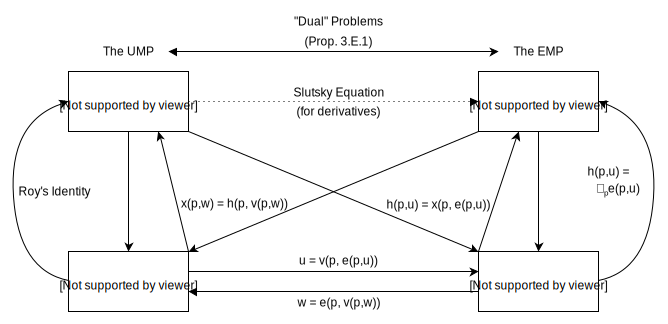
\includegraphics[width=0.9\textwidth]{./examnotes/mwg3d3.pdf}
%\includegraphics[width=0.9\textwidth]{./examnotes/dualityrelations}


\newpage

\section{Applied Consumer Theory}
\label{sec:appl-cons-theory}



\subsection{Welfare Comparisons}
\label{sec:welfare-comparisons}

Note: in what follows, the superscripts indicate time periods, while
the subscripts denote individual goods. Hence $p^x_y$ would be the
price for good $y$ in period $x$.

\begin{definition}[Equavalent Variation]
  Let $u^0 = v(p^0, w)$ and $u^1 = v(p^1, w)$. Then the equivalent
  variation EV is
  \[
  EV(p^0, p^1, w) = e(p^0, u^1) - e(p^0, u^0) = e(p^0, u^1) - w
  \]
  (note that $e(p^0, u^0) = e(p^1, u^1) = w$). 

  This can be thought of as the change in the consumer's wealth that
  would be equivalent to the price change. That is, she would be
  indifferent between a price change from $p^0 \to p^1$ and a wealth
  change $EV(p^0, p^1, w)$, which of course can be negative.
\end{definition}

\begin{definition}[Compensating Variation]
  Let $u^0 = v(p^0, w)$ and $u^1 = v(p^1, w)$. Then the compensating
  variation CV is
  \[
  CV(p^0, p^1, w) = e(p^1, u^1) - e(p^1, u^0) = w - e(p^1, u^0)
  \]
  (note that $e(p^0, u^0) = e(p^1, u^1) = w$). 

  This can be thought of as the net revenue of the planner who must
  compensate the consumer for the price change after it occurs, to
  keep her utility exactly $u^0$ (again, this could be negative).
\end{definition}

\begin{theorem}[Hicksian-Expenditure Theorem]
  Suppose only the price of good $1$ changes, ceteris paribus, then
  \[
  EV(p^0, u^0, w) 
  = -\int_{p_1^0}^{p_1^1} h_1(p_1, \bar p_{-1}, u^1) dp_1
  \]
  and
  \[
  CV(p^0, u^0, w) 
  = -\int_{p_1^0}^{p_1^1} h_1(p_1, \bar p_{-1}, u^0) dp_1
  \]
  where $\bar p_{-1}$ indicates the prices of all other goods, which
  are not changing.
  
\end{theorem}

To estimate the benefit of a new good we just take the above integrals
out to $\infty$ (or some high price where demand would be zero).

The difficulties with the above is that they rely upon Hicksian
demand, which we can't observe. So we have three tricks we can use to
make welfare analysis tractable:

\begin{enumerate}
\item Assume no income effects in demand, i.e. $x(p, w) = x(p)$ (which
  may be true for small price changes). Then
  \[
  EV = CV = -\int_{p_1^0}^{p_1^1} x_1(p_1, \bar p_{-1}) dp_1
  \]
\item Go from Marshallian to Hicksian demand nonparametrically
  (Slutsky lets us to Marshallian to derivatives of Hicksian, so if we
  solve ODE system we can recover Hicksian)
\item Convert from Marshallian to Hicksian by imposing tractable
  functional form
\end{enumerate}


\subsection{Price Indexes}
\label{sec:price-indexes}

Setup: At $t=0$ we see price $p^0$ and consumption $x^0$.  At $t=1$ we
see price $p^1$ and consumption $x^1$.

\begin{definition}[Laspeyres Price Index]
  The Laspeyres Price Index is 
  \[
  LPI = \frac{p^1 \cdot x^0}{p^0 \cdot x^0}
  \]
\end{definition}

\begin{definition}[Paasche Price Index]
  The Paasche Price Index is 
  \[
  PPI = \frac{p^1 \cdot x^1}{p^0 \cdot x^1}
  \]
\end{definition}

\begin{prop}
  The LPI overstates inflation:
  \[
  \frac{p^1 \cdot x^0}{p^0 \cdot x^0}
  \geq \frac{e(p^1, u^0)}{e(p^0, u^0)}
  \]

  The PPI understates inflation:
  \[
  \frac{p^1 \cdot x^1}{p^0 \cdot x^1}
  \leq \frac{e(p^1, u^1)}{e(p^0, u^1)}
  \]
\end{prop}

That is, the problem with both is that each has to fix consumption
bundles, so neither allows substitution that makes consumers weakly
better off in the EMP. Ideally we would just measure Hicksian
expenditure changes, but of course we can never do so.

\begin{definition}[Fisher Ideal Index]
  The Fisher Ideal Index is given by
  \[
  FII = \sqrt{ LPI \cdot PPI }
  \]
\end{definition}


\subsection{Choosing Functional Forms}
\label{sec:choos-funct-forms}


To generate simpler functional forms, we often take one of two
approaches:

\begin{enumerate}
\item Restrict preferences - impose that demand within group of goods
  is independent of prices outside the group. Thus the consumer is
  viewed as performing two step budgeting -- first allocate group
  expenditures and then within-group expenditures.
\item Restrict price movements - assume prices within group move
  proportionately. This is related to the problem set question about
  composite goods.
\end{enumerate}


\subsection{Integrability}
\label{sec:integrability}

If we observe a set of demand functions, a natural question would be
whether they are consistent with utility maximization. We already know
that rationality implies
\begin{enumerate}
\item Marshallian demand $x$ is homogenous of degree $0$
\item Marshallian demand $x$ satisfies Walras' law (i.e. $p \cdot
  x(p,w) = w$)
\item The Slutsky Matrix is symmetric and negative semidefinite
\end{enumerate}

\begin{prop}[Hurwicz-Uzawa]
  A set of continuously differentiable functions $x_i : X \times \R
  \to \R_+$ are the demand functions generated by some increasing,
  quasiconcave utility function $u$ if the satisfy Walras' law and
  have a symmetric negative semidefinite Slutsky substitution matrix.
\end{prop}

Basically, this says that we need two very simple properties on $x$ to
ensure that we are playing by the ``rules'' of micro -- i.e. that
utility analysis is appropriate.


\subsection{Demand Aggregation}
\label{sec:demand-aggregation}


\begin{definition}[Homothetic Preferences]
  Preferences are homothetic if $\forall x, y, \alpha > 0$,
  \[
  x \succeq y \implies \alpha x \succeq \alpha y
  \]
\end{definition}

\begin{prop}
  Homothetic preferences admit representation $u(x) = f(x)$ where
  $f(\alpha x) = \alpha f(x)$.
\end{prop}

\begin{prop}
  If preferences are homothetic, then demand is homogenous of degree
  $1$ in income
  \[
  x(p, \alpha w) = \alpha x(p,w)
  \]
  In general, then, if we let $\tilde x(p) := x(p, 1)$, then we can
  write
  \[
  x(p,w) = w \tilde x(p)
  \]

  Moreover, the income elasticity of demand is $1$, that is $\forall j,$
  \[
  \frac{\partial \log(x_j)}{\partial \log(w)} = 1
  \]
\end{prop}

\begin{theorem}[Chipman 1974]
  If individual preferences are homothetic but not necessarily
  identical, and incomes are proportional, then there exists a single
  preference ordering that generates aggregate demand.
\end{theorem}

\begin{prop}
  Aggregate demand is a function of aggregate wealth (i.e. typically
  aggregate demand is $X(p, w^1, \dots, w^N)$, and we want to know
  when we can represent it as $X(p, \sum w^i)$) only if 
  \[
  \frac{\partial x^k_i(p, w^k)}{\partial w^k}
  = \frac{\partial x^j_i(p, w^j)}{\partial w^j}
  \]
  $\forall$ goods $i$, and $\forall$ individuals $j,k$. The
  requirement is that wealth effects are the same across all
  individuals and across all wealth levels.
\end{prop}


In general, even if individuals have rational preferences that satisfy
GARP, if we aggregate agents and look only at aggregate demand, often
it will violate GARP. The easiest way to construct such an example is
to establish a satiation point for one or more of the agents.

Moreover, we generally cannot treat problems involving the
maximization over a set of agents' welfares instead as a problem
involving the maximization of the sum of their welfares. The issue
here is that the sum will depend upon the magnitudes of the individual
utilities, which themselves have arbitrary magnitudes because they can
be monotonically transformed and still represent preferences.

However, there is a very specifal case where we can do aggregation:
Gorman form. 

\subsubsection{Gorman Polar Form}
\label{sec:gorman-polar-form}


\begin{prop}[Gorman Polar Form]
  Demand is a function of aggregate wealth if and only if preferences
  represented by indirect utility functions of the form
  \[
  v^k(p, w^k) = a^k(p) + w^k \cdot b(p)
  \]
  where $k$ indexes the individual, hence $b(p)$ is uniform across
  consumers.
\end{prop}


In this case, aggregate demand is independent of the wealth
distribution, and maximizes:
\[
V(p,w) = \sum_k a^k(p) + w \cdot b(p)
\]
where $w = \sum_k w^k$ so we don't care about distribution. 

Now we can define a ``representative consumer'' who maximizes the
utilitarian social welfare function:
\[
W(u^1, \dots, u^k) = \sum_k u^k
\]
The intuition here is that there is some good with constant marginal
utility that is the same for all consumers. So regardless of wealth
each consumer will consume other goods until marginal utility drops
below $b(p)$ and then will put the remainder of wealth into the given
good. Then a representative consumer will consume each good until he
consumes the sum of individual demands, then puts the rest in the
constant marginal utility good.

And we can delve a bit more into the uniqueness proofs relating to
Gorman Form:

\begin{definition}[Quasi-Homothetic Preferences]
  Quasi-homothetic preferences give demands as
  \[
  x^k(p, w^k) = \alpha^k(p) + w^k \beta(p)
  \]
  where $\alpha^k$ is a person specific function but $\beta$ is
  common/identical across people.

  The aggregate demand for quasi-homothetic preferences itself
  quasi-homothetic, and is given by
  \[
  X(p,w) = \alpha(p) + w \cdot \beta(p)
  \]
  where $\alpha = \sum_k \alpha^k$ and $w = \sum_k w^k$.
\end{definition}


\begin{theorem}[Gorman 1961 Polar Form]
  The expenditure function is of the form
  \[
  e(p,u) = a(p) + u \cdot b(p)
  \]
  if and only if Marshallian demand is quasi-homothetic of form
  \[
  x(p,w) = \alpha(p) + w \cdot \beta(p)
  \]
  where $a(p)$ and $b(p)$ are homogenous of degree $1$ in price and
  \[
  \beta(p) = \frac{1}{b(p)}\frac{\partial b(p)}{\partial p}
  \]
  \[
  \alpha(p) = \frac{\partial a(p)}{\partial p} - \beta(p)a(p)
  \]

  Given the expenditure function, we can derive the indirect utility
  function of the form
  \[
  v(p,w) = \frac{w - a(p)}{b(p)}
  \]
\end{theorem}



\newpage

\section{Estimating Demand}
\label{sec:estimating-demand}

No notes here. Lecture was somewhat all over the place and nothing
showed up on a problem set. Come back to this, time permitting.

\section{Monotone Methods}
\label{sec:monotone-methods}



\subsection{Motivation}
\label{sec:motivation}

We are now concerned with comparative statics, that is, given some
maximization problem
\[
\max_{x} f(x; \theta)
\]
we want to know both how the maximum value ($v$) and the maximizing
argument ($x$) depend upon $\theta$. Assuming all derivatives exist
and the solution is interior and unique (which we could get, e.g. if
$f$ is ${\cal C}^2$, and strictly convex), we can apply the implicit
function theorem since the maximizer uniquely solves
\[
f_x(x(\theta), \theta) = 0
\]
and we can say locally that
\[
\frac{\partial x(\theta)}{\partial \theta}
= - \frac{f_{x\theta}(x(\theta), \theta)}{f_{xx}(x(\theta),\theta)}
\]
but this breaks down if any of the above assumptions fails
(e.g. differentiability, convexity), and we want our analysis to be
robust to specifications that might give a different $f$. This
introduces the idea of ``Robust Comparative Statics'' which seek to
avoid calculus and find conditions which can be used even if functions
are nondifferentiable, discontinuous, or even defined on discrete
state spaces.

\subsection{Preliminaries}
\label{sec:preliminaries}

\begin{definition}[Partial Order]
  A relation $R$ that satisfies transitivity, reflexivity, and
  antisymmetry is called a partial order.
\end{definition}

\begin{definition}[Partially Ordered Set]
  A partially ordered set, or poset, is a partial order relation
  together with a set, $(X, R)$. Note that a poset does not require
  completeness.
\end{definition}

\begin{definition}[Meet]
  The meet operator is defined as follows:
  \[
  x \wedge y = \max\{z | xRz, yRz\}
  \]
\end{definition}

\begin{definition}[Join]
  The join operator is defined as follows:
  \[
  x \vee y = \min\{z | zRx, zRy\}
  \]
\end{definition}

\begin{definition}[Lattice]
  A lattice is a poset that is closed under meet and join operations.
\end{definition}

\begin{definition}[Strong Set Order]
  The strong set order is given by the binary relation
  \[
  A \succeq_S B \iff
  a \vee b \in A, \quad
  a \wedge b \in B, \quad
  \forall a \in A, \forall b \in B
  \]
\end{definition}

\begin{definition}[Increasing Differences]
  Let $f$ be a function $f : X \times \Theta \to \R$ where both $X$
  and $\Theta$ are lattices. Consider $x^H, x^L \in X$, and $\theta^H,
  \theta^L \in \Theta$ with $x^H \geq_X x^L$ and $\theta^H \geq_\Theta
  \theta^L$. Then $f$ has increasing differences if
  \[
  f(x^H, \theta^H) - f(x^L, \theta^H) \geq
  f(x^H, \theta^L) - f(x^L, \theta^L)
  \]
  this is the same as saying that the difference $f(x^H, \theta) -
  f(x^L, \theta)$ is weakly increasing in $\theta$.
\end{definition}

\begin{definition}[Supermodularity]
  Let $f$ be a function $f : X \to \R$ where $X$ is a lattice. Then
  $f$ is supermodular if
  \[
  f(x^H \vee x^L) + f(x^H \wedge x^L) \geq f(x^H) + f(x^L) \quad
  \forall x^H, x^L \in X
  \]
\end{definition}

Note: see the proofs we did regarding supermodularity on the problem
set! Those are especially useful here.

\subsection{Topkis}
\label{sec:topkis}

\begin{theorem}[Topkis Monotonicity Theorem]
  Consider an optimization problem of the form
  \[
  \max_{x} f(x, \theta)
  \]
  and let $x^*(\theta)$ be the maximizer correspondence. If $f(x,
  \theta)$ has increasing differences, then $x^*(\theta)$ is ewakly
  increasing in $\theta$.
\end{theorem}

\begin{prop}
  Define
  \[
  x^{**}(\theta) = \sup\{ \arg \max_x f(x,\theta) + g(x) \}
  \]
  Then $x^{**}(\theta)$ is weakly increasing in $\theta$ \textbf{for
    all $g$} if and only if $f$ has increasing differences.
\end{prop}

\begin{theorem}[Topkis]
  Consider an optimization problem of the form
  \[
  \max_{x \in D} f(x, \theta)
  \]
  where $D$ is a lattice (with order $\succeq_X$) and does not depend
  on $\theta$. If $f$ exhibits increasing diferences in $(x,\theta)$
  relative to $(\succeq_X, \succeq_\Theta)$ and is supermodular in $x$
  (relative to $\succeq_X$), then the optimal choice correspondence
  $x^*(\theta)$ will be increasing in the strong set order relative to
  $\succeq_X$ (where an increase in the parameter is relative to
  $\succeq_\Theta$).

  Under the above conditions, we can conclude that $\forall \theta,
  \theta' \in \Theta$ with $\theta' \succeq_\Theta \theta$ and
  $\forall x \in x^*(\theta), x' \in x^*(\theta')$,
  \[
  x \wedge x' \in x^*(\theta) \quad \text{and} \quad x \vee x' \in x^*(\theta')
  \]
\end{theorem}


\subsection{Milgrom-Shannon}
\label{sec:milgrom-shannon}

\begin{definition}[Single Crossing]
  A function $f: \R^2 \to \R$ is single crossing in $(x, \theta)$ if
  $\forall x' > x$ and $\theta' > \theta$,
  \begin{enumerate}[(i)]
  \item $f(x', \theta) - f(x, \theta) \geq 0 \implies f(x', \theta') -
    f(x, \theta') \geq 0$
  \item $f(x', \theta) - f(x, \theta) > 0 \implies f(x', \theta') -
    f(x, \theta') > 0$
  \end{enumerate}

  We say the single crossing is strict if $f(x', \theta) - f(x,
  \theta) \geq 0 \implies f(x', \theta') - f(x, \theta') > 0$.
\end{definition}

Note that unlike increasing differences, this condition is not
symmetric in the variables $(x, \theta)$.

\begin{prop}
  If $f$ has increasing differences then it is also single crossing,
  but the converse is not true.
\end{prop}

\begin{prop}[Milgrom-Shannon Monotonic Selection Theorem]
  Define
  \[
  x^*(\theta, \bar X) := \arg \max_{x \in X} f(x, \theta)
  \]
  If $f$ is single-crossing in $(x, \theta)$, then $x^*(\theta, \bar
  X)$ is weakly increasing in $\theta \; \forall \bar X \subset X$.

  Moreover, if $x^*(\theta, \bar X)$ is non-decreasing in $\theta$ for
  all finite sets $\bar X \subset \R$, then $f$ is single-crossing in
  $(x, \theta)$.
\end{prop}

The usefulness of the Monotonic Selection theorem is that we can make
a statement about comparative statics that is robust to arbitrarily
selecting/restricting the feasible set $\bar X \subset X$.

\subsection{Long Run versis Short Run Response}
\label{sec:LR-SR}

Samuelson suggested that a firm would react more to input price
changes in the long-run than in the short-run because it has more
inputs it can adjust. We take the ``short run'' to be the period when
$k$ is effectively fixed, whereas the ``long run'' allows $k$ to
vary. We can be more precise about this relationship, though.

\begin{prop}[Milgrom and Roberts]
  Suppose $X, Y = \R$ and define
  \[
  x(y, t) := \arg \max_{x \in X} F(x,y,t)
  \]
  and
  \[
  y(t) := \arg \max_{y \in Y} F(x(y, t), y, t)
  \]
  Suppose further that $F: X \times Y \times \R \to \R$ is
  supermodular, that $t, t' \in \R $ with $t' \geq t$, and that the
  maximizes described below are unique for parameter values $t$ and
  $t'$. Then
  \[
  x(y(t'), t') \geq x(y(t), t') \geq x(y(t), t)
  \]
  and
  \[
  x(y(t'), t') \geq x(y(t'), t) \geq x(y(t), t)
  \]
\end{prop}

The above may be useful to characterize long run response. For
instance, if $x$ and $y$ happen to be complements, then the objective
would be supermodular in $x$ and $y$ and the above would characterize
growth paths.

\begin{prop}[LeChatelier Principle]
  If production is $f(k,l)$ and wage $w > w_0$ increases, and if $k$
  and $l$ are always complements or always substitutes, then
  \[
  l_{LR}(w) \leq l_{SR}(w_0, w) \leq l_{LR}(w_0)
  \]
\end{prop}

Note that when we have always complements or always substitutes, we
get supermodularity, and we can apply Milgrom-Roberts, which gives the
result.

Note also that the above does not apply when we have sometimes complements
and sometimes substitutes, which would likely be the case in many
applications. For instance, perhaps capital is a complement to labor
when labor is abundant but a substitute when labor is scarce.


\section{Monopoly}
\label{sec:monopoly}







The monopoly pricing problem is
\[
\max_q \pi(q)
\]
where $\pi(q) = q \cdot P(q) - c(q)$, and we assume it to be
differentiable, concave, and having an interior solution. Thus the FOC
is
\[
q^m \cdot P'(q^m) + P(q^m) = c'(q^m)
\]

\begin{definition}[Lerner Index]
  The Lerner Index is given by
  \[
  \frac{P(q^m) - c'(q^m)}{P(q^m)}
  \]
\end{definition}

\begin{prop}[Inverse Elasticity Rule]
  The percentave markup in the monopoly model is
  \[
  \frac{P(q^m) - c'(q^m)}{P(q^m)} = - \frac{1}{\epsilon}
  \]
  where $\epsilon = \frac{dQ}{dP} \cdot \frac{P}{Q}$ is the price
  elasticity of demand.
\end{prop}


\subsection{Assumptions}
\label{sec:assumptions}

Assume that
\begin{itemize}
\item[(A1)] Indirect utility has the form
  \begin{align}
    V_i(p,w) & = \max_{q : p \cdot q \leq w} u_i(q_1, \dots, q_L) & \notag \\
    & = \max_{q_1} f_i(q_1) + [w - p_1 q_1] & \notag
  \end{align}
  which gives us that Marshallian demand has no income effect, so we
  can write $x(p)$ instead of $x(w,p)$ and we can make comparisons
  across consumers with different levels of wealth
\item[(A2)] $w_i = w_{0i} + s_i \pi(p)$ which means that firms are
  owned by consumers, where $s_i$ is consumer $i$'s share of the
  profits that the firm obtains
\end{itemize}

\subsection{Monopolist Quantity}
\label{sec:monopolist-quantity}



\begin{prop}
  Given any depand curve $P(q)$ and cost function $c(q, \theta)$, define
  \[
  q^m = \sum \arg \max_q q \cdot p(q) - c(q, \theta)
  \]
  If $c(q, \theta)$ has increasing differences, then $q^m$ is weakly
  increasing in $\theta$.
\end{prop}

\begin{prop}[Monopolistic Underprovision]
  Let
  \[
  q^{FB} = \sup \arg \max_q \int_0^q P(s) ds - c(q)
  \]
  and
  \[
  q^m = \sup \arg \max_q q \cdot P(q) - c(q)
  \]
  If $P'(q) \leq 0$ then $q^m \leq q^{FB}$.
\end{prop}



\subsection{Monopolist Quality}
\label{sec:monopolist-quality}

Suppose a monopolist chooses quality $s$ in addition to quantity, so
now we can define
\[
W(q,s) = \int_0^q P(x,s) dx - c(q,s)
\]
and
\[
\pi(q,s) = q \cdot P(q,s) - c(q,s)
\]

\begin{prop}
  Let 
  \[
  s^{FB} = \sup \arg \max_s W(q,s)
  \]
  and
  \[
  s^m(q) = \sup \arg \max_s \pi(q,s)
  \]
  If $P(q,s)$ has decreasing differences in $q$, then $s^{FB}(q) \geq
  s^m(q)$.
\end{prop}

The intuition here is that the value of quality is less for the
marginal consumer than for the average consumer. Since the monopolist
only cares about the marginal consumer but the social planner cares
about the average consumer, we get a distortion from optimum, known as
the \textbf{Spence Distortion}. On the other hand, the IO literature
notes that since the monopolist sells fewer units, the marginal
monopolist consumer has a higher value than the social planner's
marginal consumer. Thus in richer models where $q$ can vary (in the
above we've fixed $q$), this effect can offset and yield $s^m >
s^{FB}$.






\section{Externalities}
\label{sec:externalities}





\subsection{Preliminaries}
\label{sec:preliminaries}

Consumers are assumed to have utility functions that take quasilinear
form.

\begin{definition}[Quasilinear Utility]
  A utility function is quasilinear with respect to a numeraire
  commodity if it takes the form
  \[
  u_i(x_{i}, h) = g_i(x_{-1i}, h) + x_{1i}
  \]
  where $x_1$ is the numeraire and $x_{-1}$ is all other goods. Thus
  the consumer gets linear utility in the numeraire and will always
  consumer other goods only until on the margin the numeraire is
  preferred, i.e the consumption decision for other goods
  $x_{-1i}(p,h)$ is constant as a function of wealth. We can then
  write the indirect utility function as
  \[
  v_i(p,w,h) = g_i(x_{-1i}(p,h), h) + (w_i - p \cdot x_{-1i}(p, h))
  \]
  there the final term is the amount of money left over for the
  numeraire. If we then let $\phi_i(p,h) := g_i(x_{-1i}(p,h), h) - p
  \cdot x_{-1i}(p, h)$ we get indirect utility of the form
  \[
  v_i(p, w_i, h) = \phi_i(p,h) + w_i
  \]
  which, as above, has no wealth effects.
\end{definition}

We additionally assume that prices of traded goods are unaffected by
any actions within our model, so we assume $p$ is constant and
suppress its notation. That is, we denote $\phi_i(p,h)$ as
$\phi_i(h)$. We further assume that $\phi \in {\cal C}^2$ with
$\phi''_i(\cdot) < 0$. In what follows, we study a two agent model,
where the first consumer makes the choice about how much of the
externality to consume.

The first consumer chooses $h$ to solve
\[
\max_{h \geq 0} \phi_1(h)
\]
which gives, at the optimum,
\[
\phi_1'(h^*) \leq 0 \quad \text{with equality if } h^* > 0
\]
(because she cannot consume negative externality).

By contrast, any Pareto Optimal allocation $h^\circ$ would solve
\[
\max_{h \geq 0} \phi_1(h) + \phi_2(h)
\]
which gives, at the optimum
\[
\phi_1'(h^\circ) \geq -\phi_2'(h^\circ) \quad \text{with equality if } h^\circ > 0
\]

Note that unless $h^* = h^\circ = 0$, as long as $\phi_2(h) \neq 0$
the equilibrium level of $h$ is not Pareto efficient.

\subsection{Solutions to the Externality Problem}
\label{sec:solut-extern-probl}

\subsubsection{Quotas}

Suppose that $h$ generates a negative external effect, so that
$h^\circ < h^*$. Then the government could impose that $h \leq
h^\circ$ and indeed consumer one would set the level of the
externality at $h^\circ$.

\subsubsection{Taxes}

The government could either tax per unit of $h$ or subsidize per unit
reduction of $h$ (on consumer $1$). Suppose consumer $1$ were forced
to pay a tax $t_h$ per unit of $h$. Then she maximizes
\[
\max_{h \geq 0} \phi_1(h) - t_h \cdot h
\]
thus if $t_h = - \phi_2'(h^\circ) > 0$, the competitive equilibrium
will be $\phi_1'(h) = t_h = -\phi_2'(h)$, which is satisfied by
$h^\circ$. This type of tax is known as a Pigouvian corrective tax. In
particular, the optimality-resotoring tax is set at the level of the
marginal externality at the optimal solution.

We could also have used a subsidy above, which has consumer $1$
maximize
\[
\max_h \phi_1(h) + s_h(h^\circ - h)
\]
which is effectively a lump sum transfer combined with a tax, and can
be optimality restoring.

Note that in many cases the government lacks sufficient information
about the costs and benefits of the externality, and also sometimes is
unable to directly tax the externality and instead must apply quotas
or taxes to total output. In these cases, we often cannot achieve an
efficient outcome.

\subsection{Coase}
\label{sec:coase}

Coase viewed the externality problem as arising from a combination of
\begin{enumerate}[(i)]
\item lack of clearly specified property rights
\item transaction costs
\end{enumerate}


\begin{theorem}[Coase]
  If property rights are clearly specified and there are no
  transaction costs, bargaining will lead to an efficient outcome no
  matter how the rights are allocated.
\end{theorem}

Note that this does not say that distribution is unaffected, just that
an efficient outcome is attained.

As an example, consider allocating to consumer $2$ rights to
externality free environment. She can make a take it or leave it offer
of payment $T$ (that consumer $1$ would make to her) in order for $1$
to have the rights to consume the externality at level $h$ (but
consumer $1$ may reject the deal). Thus consumer $2$ maximizes
\[
\max_{h, T} \phi_2(h) + T \quad s.t. \quad \phi_1(h) - T \geq \phi_1(0)
\]
but since the constraint is binding, we can solve for $T$ and plug in
to get the reframed problem for consumer $1$:
\[
\max_h \phi_2(h) + \phi_1(h) - \phi_1(0)
\]
which yields the FOC that guarantees the socially optimal level.

If we switched the property rights, such that consumer $1$ has the
right to generate as much $h$ as she wants. Still consumer $2$ makes a
take it or leave it offer to consumer $1$ offering payment $T$ in
order to reduce the externality to $h$. Then consumer $1$'s problem is
\[
\max_{h,T} \phi_2(h) - T \quad s.t. \quad \phi_1(h) + T \geq \phi_1(h^*)
\]
again the constraint is binding so we can rewrite the above to
\[
\max_h \phi_2(h) - (\phi_1(h^*) - \phi_1(h))
\]
which again gives FOCs that generate the social optimum.

Note that in special case where two parties are firms, another
solution to let the two firms merge. The resulting firm would fully
internalize the externality when maximizing profits. Note also that
unlike the tax and quota schemes, Coase’s approach only requires that
the consumers know each others preferences, and not government.



\subsection{Myerson Satterthwaite}
\label{sec:myers-satt}

Suppose $h$ is now a discrete choice, $\{0, \bar h\}$ and $\theta,
\eta$ random variables that influence each agent's utility, i.e.
$\phi_1(h; \theta)$ and $\phi_2(h; \eta)$. Then we can define
\[
b(\phi) = \phi_1(\bar h; \theta) - \phi_1(0; \theta) > 0
\]
and
\[
s(\phi) = \phi_2(0; \eta) - \phi_2(\bar h; \eta) > 0
\]
thus when $b(\theta) > s(\eta)$ the Pareto optimal level is $\bar
h$. Then if we let $G(b)$ and $F(s)$ be the CDFs induced by $\theta,
\eta$, and we give consumer $2$ the right to an externality free
environment, then she will always choose $h=0$ which is inefficient if
$b(\theta) > s(\eta)$.

Suppose now we allow consumer $1$ to offer a transfer $T$ for the
ability to consume $\bar h$. And assume each consumer knows their own
values but not the other person's. Under this transfer, we know
consumer $2$ will agree iff $T \geq s$, the probability of which is
$F(T)$. Hence consumer $1$ solves
\[
\max_T \underbrace{F(T)}_{P(\text{2 accepts})}
\underbrace{(b - T)}_{\text{payoff}}
\]
and will make an offer $T$ that is less than $b$ (positive profits)
but is greater than the minimum value of $s$ (otherwise agent $2$
never accepts). But suppose given the realization of $\eta$ that 
\[
b(\theta) > s(\eta) > T
\]
then in this case the efficient level is $\bar h$ since $b(\theta) >
s(\eta)$, but the offer will be rejected. Hence there is a positive
probability of inefficiency in this context even with transfers.

\begin{prop}[Myerson-Sattherthwaite]
  No bargaining procedure can lead to an efficient outcome for all
  values of $b$ and $s$ when they are private information and
  independently distributed.
\end{prop}

\subsection{Missing Markets}
\label{sec:missing-markets}

Suppose we can construct a competitive market for the externality
(which may not always be possible), with price per unit $p_h$. Then
consumer $1$ buys rights to $h$ to solve
\[
\max_{h_1} \phi_1(h_1) - p_h h_1
\]
and consumer $2$ sells rights to $h$ to solve
\[
\max_{h_2} \phi_2(h_2) + p_h h_2
\]
which gives the two FOCS
\[
\phi_1'(h_1) = p_h \quad \text{and} \quad \phi_2'(h_2) = -p_h
\]
which clearly generateds the Pareto Optimal level of the externality
in equilibrium (when we impose $h_1 = h_2 = h^{**}$. 


\subsection{Prices versus Quantities}
\label{sec:pric-vers-quant}



We saw earlier that taxes and quotas generated efficient levels of the
externality. Yet when we add uncertainty, the two are not equivalent
any longer.

\subsubsection{Setup}


Suppose that firms generate externalities (and can be regulated) and
consumers derive negative benefit from the externalities. Suppose
there is uncertainty in the value of the externality, with the firm's
profit given by $\pi(h, \theta)$ and the consumer's utility $\phi(h,
\eta)$, where $\theta, \eta$ are random variables that are privately
observed. However, the CDFs of $\theta, \eta$ are publicly known
\textit{ex ante}. We assume that $\pi(h,\theta)$ and $\phi(h, \eta)$
are strictly concave in $h, \forall \theta, \eta$.

If the government could obesrve realizations of $\theta$ and $\eta$
and make its decision \textit{ex post} then it would get the first
best quota
\[
h^\circ(\theta, \eta) = \arg \max_h \{ \pi(h, \theta) + \phi(h, \eta) \}
\]
or tax
\[
t_h^\circ(\theta, \eta) 
= \frac{\partial \pi(h^\circ(\theta, \eta), \theta)}{\partial h}
= \frac{\partial \phi(h^\circ(\theta, \eta), \theta)}{\partial h}
\]
these are the first best solutions, and form the basis of
comparison. Both will yield equilibrium externality levels of
$h^\circ$, given above.


However, the government is often unable to observe these values, or at
least unable to craft policy in response to every realization. So now
we assume the government must commit in advance to a tax or quota
policy, knowing only the \textit{ex ante} distributions of $\theta$
and $\eta$. 

We must first consider the firm's response to taxes or quantity
regulation. In the case of quantity regulation with quata $\hat h$,
the firm solves
\[
\max_{h \geq 0} \pi(h, \theta) \quad s.t. \quad h \leq \hat h
\]
and we denote the optimal choice $h^q(\hat h, \theta)$. In the case of
a tax, the firm solves
\[
\max_{h \geq 0} \phi(h, \theta) - th
\]
and we denote the optimal choice $h^t(t, \theta)$. 


We now consider the optimal tax or quota from the government's
perspective. Under quota regulation the planner solves
\[
\hat h^* = \arg \max_{\hat h}
E \left[ \pi(h^q(\hat h, \theta), \theta) 
+ \phi(h^q(\hat h, \theta), \eta) \right]
\]
and in the case of taxation the planner solves
\[
t^* = \arg \max_t
E \left[ \pi(h^t(t, \theta), \theta)
+ \phi(h^t(t, \theta), \eta) \right]
\]

Note that these optimizations are performed in expectation, so in
general it will not be the case that for any given realization they
are first best. Thus we will want to study the loss in aggregate
surplus under given realizations of $(\theta, \eta)$. In the case of a
quota, the loss is
\[
(\pi(h^q(\hat h, \theta), \theta) + \phi(h^q(\hat h, \theta), \eta))
- (\pi(h^\circ(\theta, \eta), \theta) + \phi(h^\circ(\theta, \eta), \eta))
\]
which is equivalent to
\[
\int_{h^\circ(\theta, \eta)}^{h^q(\hat h, \theta)}
\left( \frac{\partial \pi(h, \theta)}{\partial h}
+ \frac{\partial \phi(h, \eta)}{\partial h} \right) dh
\]
and in the case of a tax the loss is
\[
(\pi(h^t(t, \theta), \theta) + \phi(h^t(t, \theta), \eta))
- (\pi(h^\circ(\theta, \eta), \theta) + \phi(h^\circ(\theta, \eta), \eta))
\]
which is equivalent to
\[
\int_{h^\circ(\theta, \eta)}^{h^t(t, \theta)}
\left( \frac{\partial \pi(h, \theta)}{\partial h}
+ \frac{\partial \phi(h, \eta)}{\partial h} \right) dh
\]


Weitzman makes functional form simplifications which are similar to
second order Taylor approximations around the point $\hat h^*$ to give
\[
\pi(h, \theta) 
= b(\theta) + (\pi' + \beta(\theta))(h - \hat h^*) + \frac{\pi''}{2}(h - \hat h^*)^2
\]
and
\[
\phi(h, \theta) 
= a(\eta) + (\phi' + \alpha(\eta))(h - \hat h^*) + \frac{\phi''}{2}(h - \hat h^*)^2
\]
with
\[
E[\beta(\theta)] = E[\alpha(\eta)] = 0
\]
and he defines the advantage of a tax over quota regulation as
\[
\Delta 
= E[\{ \pi(h^t(t, \theta), \theta) + \phi(h^t(t, \theta), \eta) \}
- \{ \pi(\hat h, \theta) + \phi(\hat h, \eta) \} ]
\]
to give the result

\begin{prop}[Weitzman]
  The benefit of price regulation over quantity regulation, as given
  above, is
  \[
  \Delta = \frac{\sigma^2}{2(\phi'')^2}(\pi'' - \phi'') = (+)[(-) + (+)]
  \]
  where $\sigma^2$ is the variance of $\phi$ at $\hat h$. This means
  that price regulation is better than quantity regulation if and only
  if $\phi'' > |\pi''|$. The intuition is that prices are better when
  the firm faces more uncertainty, since they allow variability here,
  while quantities are better when the consumer faces more
  uncertainty, since it imposes a hard cap on the externality.
\end{prop}

\subsection{Equilibrium Number of Boats}
\label{sec:equil-numb-boats}

This is an example that is addressed both in lecture and in the
problem set, so see either for full exposition and solution. Basically
the planner cares about average cost of sending out additional boats
while the individual fisherman only care about whether they can make
positive profit on the margin (they don't internalize the externality
that they impose on the other fishermen by reducing the number of fish
per capita or something). Thus the planner's number of boats is always
smaller than if we let the fishermen decide on their own.



** TODO: do we need to know Lindahl equilibrium? I think it was on a problem set, and is addressed briefly on MWG pp. 363--364 **

** TODO: write up definitions of depletable and non-depletable externalities MWG section 11.D **






\section{General Equilibrium: Main Issues}
\label{sec:main-issues}






\subsection{Setup}

We study here an exchange economy with no production. There are a
finite number of agents $i$ and commodities $l$. A consumption bundle
is a bundle of commodities $x \in \R^L_+$. Each agent has an endowment
$\omega^i \in \R^L_+$ and a utility function $u^i : \R^L_+ \to \R$. We
denote an economy as a set of endowments and utlity functions
\[
{\cal E} = \{(u^i, \omega^i)\}
\]
thus at prices $p$ the agent has a budget set $B^i(p) = \{x : p \cdot
x \leq p \cdot \omega^i\}$ hence each agent solves
\[
\max_{x \in B^i(p)} u^i(x)
\]

\begin{definition}[Walrasian Equilibrium]
  A Walrasian equilibrium for economy ${\cal E}$ is a pair $(p,
  \{x^i\}_{i \in I})$ such that
  \begin{enumerate}[(i)]
  \item Agents maximize utility under prevailing prices:
    \[
    \forall i \in I, x^i \in \arg \max_{x \in B^i(p)} u^i(x)
    \]
  \item Markets clear for each good:
    \[
    \forall l \in {\cal L}, \sum_{i \in I} x^i_l = \sum_{i \in I} \omega^i_l
    \]
  \end{enumerate}
\end{definition}

\begin{definition}
  An allocation $\{x^i\}_{i \in I}$ is feasible if
  \[
  \forall l \in {\cal L}, \sum_{i \in I} x^i_l \leq \sum_{i \in I} \omega^i_l
  \]
\end{definition}

Note that the equilibrium only cares about relative, not absolute
prices.

\begin{prop}
  If the market for one clears, then the other markets clear as well.
\end{prop}

\begin{definition}[Pareto Optimal]
  Given an economy ${\cal E}$, a feasible allocation $x$ is Pareto
  optimal/efficient if there is no other feasible allocation $\hat x$
  such that
  \begin{enumerate}[(i)]
  \item $\forall i \in I, u^i(\hat x^i) \geq u^i(x^i)$
  \item $\exists i \in I: u^i(\hat x^i) > u^i(x^i)$
  \end{enumerate}
\end{definition}

\subsection{The Four Assumptions}
\label{sec:four-assumptions}

We make the following assumptions on preferences on each agent $i$,
termed \textbf{\textit{the four assumptions}}:

\begin{enumerate}
\item $u^i$ is continuous
\item $u^i$ is increasing in $x$
\item $u^i$ is concave
\item $\omega^i >> 0$
\end{enumerate}

The first three are similar to what we've always used. The last is
important, new, and strong. It can be used to eliminate odd corner
solutions.


\subsection{A $2 \times 2$ Exchange Economy}
\label{sec:2-times-2}


For simplicity we now study the pure exchange economy described above
in the limited case where there are two consumers and two goods. This
lends itself to easy study by use of an Edgeworth box. We use the
following definitions in the context of this exchange economy

\begin{definition}[Allocation]
  An allocation $x$ assigns a nonnegative consumption vector to each consumer
  \[
  x = (x^1, x^2) = ((x^1_1, x^1_2), (x^2_1, x^2_2))
  \]
\end{definition}

\begin{definition}[Feasible]
  An allocation is feasible if $\forall l = 1, 2$
  \[
  x^1_l + x^2_l \leq \omega^1_l + \omega^2_l
  \]
\end{definition}

\begin{definition}[Non-Wasteful]
  An allocation is nonwasteful if
  \[
  x^1 + x^2 = \omega
  \]
\end{definition}

\begin{definition}[Budget Set]
  The budget set for consumer $i$ is given by
  \[
  B^i(p) = \{x \in \R^2_+: p \cdot x \leq p \cdot \omega^i\}
  \]
  where, in general, the budget set may extend outside of the
  Edgeworth box.
\end{definition}

\begin{definition}[Offer Curve]
  Given a fixed exchange economy ${\cal E}$ (fixed endowments and
  utility functions), the offer curve for consumer $i$ is generated by
  adjusting $p$ and for each $p$ tracing out the feasible allocation
  that maximizes consuemr $i$'s utility, thus generating a curve. 
\end{definition}

Note that the consumer's endowment will always be affordable, so the
offer curve must lie above the indifference curve passing through the
endowment.

\begin{definition}[Excess Demand]
  Total agent demand for a commodity is greater than what is available
  in the economy (corner solution).
\end{definition}

\begin{definition}[Pareto Set]
  Allocations where indifference curves of the two consumers are
  tangent. They are characterized by
  \[
  \frac{
    \frac{\partial u^1}{\partial x^1}
  } {
    \frac{\partial u^1}{\partial x^2}
  }
  (x^1)
  =
  \frac{
    \frac{\partial u^2}{\partial x^1}
  } {
    \frac{\partial u^2}{\partial x^2}
  } (\omega - x^1)
  \]
\end{definition}

\begin{definition}[Contract Curve]
  The section of the Pareto set where each consumer does at least as
  well as her initial endowment.
\end{definition}

\subsection{Welfare Theorems}
\label{sec:welfare-theorems}



\begin{theorem}[First Welfare Theorem]
  Let $(p, \{x^i\}_{i \in I})$ be a Walrasian equilibrium for economy
  ${\cal E}$. If utility is increasing, then allocation $\{x^i\}_{i
    \in I}$ is Pareto optimal.
\end{theorem}

This says that even without explicit coordination, decentralized
markets where agents simply maximize their utilities given prices are
efficient. However, it should be emphasized that the model has a
number of heroic assumptions; e.g., agents face the same prices,
agents are price takers, markets exist for all goods, and we haven’t
said where prices come from.

\begin{theorem}[Second Welfare Theorem]
  Let ${\cal E}$ satisfy our four assumptions. If $\{\omega^i\}_{i \in
    I}$ is Pareto optimal, then $\exists p \in \R^L_+$ such that $(p,
  \{\omega^i\}_{i \in I}$ is a Walrasian equilibrium for ${\cal E}$.
\end{theorem}

Note that the SWT does not say that starting from a given endowment,
every Pareto optimal allocation is a Walrasian equilibrium; rather, it
says if we start from a given endowment, then for any Pareto optimal
allocation, there is a way to redistribute resources and prices that
makes the allocation a Walrasian equilibrium outcome. That is, once we
find an efficient allocation, we could support it with a price
equilibrium. But in that case, why not simply implement it directly
without prices?


We now proceed with a sketch of the proofs for the Welfare
Theorems. We use the four assumptions given above, and additionally
make the simplifying assumption that $\nabla u^i(x^i) > 0$ and that
$u^i(0) = 0$. 

\begin{definition}[Utility Possibility Set]
  The utility possibility set (UPS) is given by
  \[
  {\cal U} = \{u^1(x^1), \dots, u^l(x^l) : \sum x^i \leq \sum \omega^i \}
  \]
\end{definition}

Note that Pareto optimal allocations are those on the ``northeast''
frontier of the UPS. Now consider the following program
\begin{align}
  \max_{x^1} u^1(x^1) \quad s.t. & \quad u^i(x^i) \geq \bar u^i 
  & i = 2, \dots, I \notag \\
  & \quad \sum x^i_l \leq \sum \omega^i_l & l = 1, \dots, L \notag
\end{align}
then Pareto optimal allocations solve this program for different
values of $(\bar u^2, \dots, \bar u^l) \geq 0$. That is, we maximize
the utility of our first consumer subject to other consumers getting
at least some prespecificed level of utility each. Since we can vary
the required levels $\bar u$ we can recover the full set of Pareto
optimal outcomes. If we restrict our attention to $\bar u >> 0$, then
under our first three assumptions the utility constraints are binding;
if they weren't, we could reduce allocation to the slack constraint
and give it to consumer $1$ whose utility is increasing in $x^1$. Then
we can apply KT to get the Lagrangian
\[
\sum_{i \in I} \lambda^iu^i(x^i) 
+ \sum_{l \in L} \mu_l \left( \sum_{i \in I}\omega^i_l -  \sum_{i \in I} x^i_l \right)
\]
where by convention $\lambda^1 = 1$. And since all constraints bind,
$\lambda^i > 0$ and $\mu_l > 0$. So our FOCs are
\begin{enumerate}
\item $\lambda^i \frac{\partial u^i(x^i)}{\partial x^i_l} - \mu_l \leq 0$
\item $\left(\lambda^i \frac{\partial u^i(x^i)}{\partial x^i_l} -
    \mu_l\right)x^i_l \leq 0$
\item $x^i_l \geq 0$
\item $\sum_i x^i = \sum_i \omega^i$
\end{enumerate}
(note that we could also interpret this Lagrangian as arising from
maximizing a social welfare function subject to resource constraints).

Now we turn our attention not to Pareto optimal outcomes, but
competitive outcomes under Walrasian equilibria. Each consumer solves
the UMP under prices $p$:
\[
\max_{x^i} u^i(x^i) \quad s.t. \quad p \cdot x^i \leq p \cdot \omega^i
\]
which is a constrained optimization problem, so we use KT and let
$\gamma^i$ be the multiplier on the budget constraint. Then under
the FOCs are
\begin{enumerate}
\item $\frac{\partial u^i(x^i)}{\partial x^i_l} - \gamma^ip_l \leq 0$
\item $\left(\frac{\partial u^i(x^i)}{\partial x^i_l} -
    \gamma^ip_l\right)x^l_l = 0$
\item $x^i_l \geq 0$
\end{enumerate}
then $x$ can be supported as a price equilibrium if and only if we can
find vectors $p$ and $\gamma$ such that the above KT conditions
hold. But these KT conditions are exactly the same as on the Pareto
optimal outcome! This observation implies the two
welfare theorems.

\textbf{Proof of FWT.} If $\omega$ and $p$ are given and each agent
solves UMP, then at consumption bundles $\{x^i\}$ the UMP KT
conditions hold. Then if we let $\bar u^i = u^i(x^i), i = 2, \dots,
I$, and we define $\mu_l = p_l$ and $\lambda^i = (\gamma^i)^{-1}$ then
the KT conditions for the Pareto problem are also met. Hence any
Walrasian equilibrium is Pareto optimal.

\textbf{Proof of SWT.} If KT condtions for the Pareto program are
satisfied then we can define prices $p_l = \mu_l$ and multipliers
$\gamma^i = (\lambda^i)^{-1}$ and we therefore meet the KT conditions
for the UMP, hence $(p, x)$ Walrasian equilibrium with endowment
$\omega = x$.

Note that the above proof of the SWT gives the interpretation that the
supporting price vector $p$ is the vector of shadow prices $\mu$ on
the aggregate endowment of each good.




\subsection{Robinson-Crusoe: One-Producer, One-Consumer Economy}
\label{sec:robinson-crusoe}

Setup:
\begin{itemize}
\item two goods, leisure (1) and consumption good (2)
\item wage for labor $w$ and price of consumption good $p$ taken as
  exogenous
\item single consumer with endowment $\bar L$ of leisure and $0$ of
  the consumption good
\item single firm with strictly concave technology $f(z)$
\item consumer owns the firm and receives all profits
\end{itemize}

The firm therefore solves
\[
\max_z p f(z) - wz
\]
and we denote the optimal labor demand $z(p, w)$, the optimal output
level $q(p,w)$, and the optimal profits $\pi(p,w)$. 

The consumer solves
\[
\max_{x_1, x_2} u(x_1, x_2) \quad s.t. \quad px_2 \leq w(\bar L - x_1) + \pi(p, w)
\]

A Walrasian equilibrium in this economy is a price vector $(p^*, w^*)$
at which both markets clear, i.e.
\begin{align}
x_2(p^8, w^*) &= q(p^*, w^*) & \text{consumption market clears} \notag \\
z(p^*, w^*) = \bar L - x_1(p^*, w^*) & \text{labor market clears} \notag
\end{align}



\subsection{A $2 \times 2$ Production Economy}
\label{sec:2-times-2-prod}

Setup:

\begin{itemize}
\item $2$ goods and $2$ factors
  \begin{itemize}
  \item each firm produces a single good, i.e. two firms
  \item factor $1$ is labor, factor $2$ capital, with input prices $w$
    and $r$, respectively
  \item total endowment is $L$ and $K$, respectively
  \item goods prices $p_1, p_2$
  \end{itemize}
\item each firm has constant returns to scale (CRS) technology,
  i.e. $f(\lambda k, \lambda l) = \lambda f(k, l)$ and $c(w,r,q) = q
  c(w,r,1)$

\end{itemize}

Each firm $j$ then solves
\[
\max_{k_j, l_j} p_j f_j(k_j, l_j) - c_j(w, r, q_j)
\]
and under CRS the FOC is
\[
p = \frac{\partial c(w,r,q)}{\partial q} 
= \frac{\partial [qc(w,r,1)]}{\partial q} = c(w,r,1)
\]
however, this does not gives us a level of output (due to CRS). So we
move to per-unit analysis, and we get total cost for firm $j$ to
produce $q^j$ units is
\[
C^j(w, r, q^j) = 
\underbrace{\min\{wl + rk \; | \; f(k, l) \geq 1 \} }_{c^j(w,r) = \text{"unit cost"}}
\cdot q^j
\]
then we can denote $a^j_l(w,r)$ and $a^j_k(w,r)$ to be the per-unit
factor demands at given factor prices that solve the above cost
minimization problem.

\begin{lemma}[Shepard's Lemma]
  Under the above,
  \[
  \frac{\partial c^j(w,r)}{\partial w} = a^j_l(w,r)
  \]
  and
  \[
  \frac{\partial c^j(w,r)}{\partial r} = a^j_k(w,r)
  \]
\end{lemma}

For a given quantity $q^j$, firm $j$ therefore uses $a^j_lq^j$ units
of labor. ``Full employment conditions'' mandate that all available
labor and capital is employed, that is, with two firms:
\[
a^1_l q^1 + a^2_lq^2 = L
\]
and
\[
a^1_k q^1 + a^2_k q^2 = K
\]


\begin{definition}[Specialization]
  If only one good is produced is equilibrium, we say the economy is
  specialized.
\end{definition}

If we assume that there is no specialization and both goods are
produced, we have an interior solution and equilibrium factor prices
are determined by the FOCs
\[
p^1 = c^1(c^*, r^*) \quad p^2 = c^2(c^*, r^*)
\]


\begin{definition}[Intensive Production]
  We say that production of good $1$ is relative more intensive in
  labor than production of good $2$ if 
  \[
  \frac{a^1_l(w,r)}{a^2_l(w,r)} > \frac{a^1_k(w,r)}{a^2_k(w,r)}
  \quad \forall (w,r)
  \]
\end{definition}


\begin{theorem}[Samuelson 1949]
  Two countries with identical technologies facing the same product
  prices will have the same factor prices even if factor endowment
  differs (version of ``factor price equalization (FPE)'' theory by
  Samuelson).
\end{theorem}

\begin{theorem}[Stolper-Samuelson Theorem]
  Under the above economy, if $p_j$ increases, the equilibrium price
  of the factor more intensively used in the production of good $j$
  increases, while the price of the other factor decreases (assuming
  interior equilibria both before and after the price change).
\end{theorem}

\begin{theorem}[Rybcszynski Theorem]
  If the endowment of a factor increases, then the production of the
  good that uses this factor relatively more intensively increases,
  while the production of the other good decreases (assuming interior
  equilibria both before and after the price change).
\end{theorem}



\subsection{Public Goods}
\label{sec:public-goods}

We now return to Chapter 11 in MWG for discussion of public goods.

\begin{definition}[Public Good]
  A public good is a good for which use of a unit by one consumer does
  not preclude its use by others.
\end{definition}

\begin{definition}[Non-depletable/non-rivalrous/public]
  A good is non-depletable if one agent's consumption of the good does
  not subtract from any other agent's consumption of said good.
\end{definition}

\begin{definition}[Excludability]
  A public good is non-excludable if, once it has been provided to one
  consumer, it is impossible (or prohibitively costly) to prevent
  others from consuming it (e.g. a lighthouse). 
\end{definition}

\begin{definition}[Impure Public Good]
  An impure public good, or public good with congestion, is a good
  that can be shared, but eventually additional consumers impose
  negative externalities on others (e.g. a swimming pool).
\end{definition}

Public goods are interesting to study because common sense suggests
that they will be under-provided by the usual market mechanism.

\subsubsection{Neo-Classical Theory of Public Goods}

Setup:
\begin{itemize}
\item $n$ consumers indexed by $i = 1, \dots, n$
\item two goods -- a numeraire private good $x$ and public good $G$
\item consumer $i$ has utility $u^i(x^i, G)$ which is differentiable,
  increasing in both arguments, quasi-concave, and $u^i(x^i, 0) > 0$
  (which guarantees an interior solution)
\item consumer $i$ has endowment of numeraire $w^i$, and we denote $W
  = \sum_i w^i$
\item public good endowment is zero
\item $G = f(z)$, where $z$ is total units of private goods used as
  inputs
\end{itemize}

\begin{definition}[Allocation]
  An allocation for this community consists of
  \begin{enumerate}[(i)]
  \item A level public good $G$
  \item An allocation of private goods $x = (x^1, \dots, x^n)$
  \end{enumerate}
\end{definition}

\begin{definition}[Feasible]
  An allocation for this community is feasible if $\exists z \geq 0$ s.t.
  \begin{enumerate}[(i)]
  \item $z + \sum_i x^i \leq W$
  \item $G \leq f(z)$
  \end{enumerate}
\end{definition}


\begin{definition}[Pareto Optimality/Lindahl-Samuelson Condition]
  An allocation $(x, G)$ is Pareto optimal if and only if
  \[
  \sum_{i=1}^n 
  \frac{
    \frac{\partial u^i(x^i, g)}{\partial G}
  } {
    \frac{\partial u^i(x^i, G)}{\partial x^i}
  }
   = \frac{1}{f'(z)}
  \]
\end{definition}

The above is know as the \textit{Lindahl-Samuelson Condition}. It says
that the sum of the marginal rates of substitutions between the agents
is equal to the amount of private good required to produce an
additional unit of the public good.




\subsubsection{Market Provision of Public Goods}

Setup:
\begin{itemize}
\item public good has price $p$
\item agents choose how much to buy, $g^i$
\item single price-taking, profit-maximizing firm that produces public
  good
\end{itemize}

The issue is that we have a \textit{strategic problem}, since the
amount demanded by each agent depends on what she expects other agents
to demand (note that all agents uniformly enjoy total $G$ that the
firm produces).

\begin{definition}[Competitive Equilibrium]
  A competitive equilibrium in this contetx consists of $p^*$ and $G^*
  = (g^{1*}, \dots, g^{n*})$ s.t.
  \begin{enumerate}[(i)]
  \item Each agent's choice $g^i$ maximizes utility given $p^*$ and
    $g^*_{-i}$
  \item The firm optimizes
    \[
    \max_{z \geq 0} p^* f(z) - z
    \]
    which is equivalent to
    \[
    p^* = \frac{1}{f'(f^{-1}(\sum g^{i*})}
    \]
  \end{enumerate}

\end{definition}


\begin{prop}
  In the above competitive equilibrium, there is under-provision of
  the public good relative to the level prescribed by the Lindahl-Samuelson
  condition.
\end{prop}

The intuition is that we have a \textit{free-rider} problem, i.e. each
agent free rides on others' provisions, and does not consider the
benefit to other agents of the output that she purchased.

\subsubsection{Lindahl Equilibrium and Personalized Prices}

In this model, we assume that somehow the public good is excludable
and can be offered to each agent at a different ``personalized
price.'' We also assume that agents own the firm that produces the
public good, with agent $i$'s share in the firm's profits given by
$s^i \in [0,1]$ with $\sum_i s^i = 1$.

\begin{definition}[Personalized Price]
  An agent's personalized price is a price $p^i$ that the agent faces
  to purchase one unit of the public good, and can differ across
  agents.
\end{definition}

We can select personalized prices such that agents all agree on the
level of the public good $G$. This fictitious economy has $n+1$ goods,
the private good (which is the same for everybody) plus the $n$
personalized public goods.


\begin{definition}[Lindahl Equilibrium]
  A Lindahl equilibrium is a vector $p^* = (p^{1*}, \dots, p^{n*})$
  and allocation $x^{1*}, \dots, x^{n*}, G^*$ s.t.
  \begin{enumerate}[(i)]
  \item The firm maximizes total profits:
    \[
    G^* = \arg \max_{G \geq 0} \left(\sum_i p^{i*}\right)G - f^{-1}(G)
    \]
  \item Consumers maximize utility subject to their budget constaints:
    \[
    (x^{i*}, G^*) = \arg \max_{x^i, G} u^i(x^i, G)
    \quad s.t. \quad  x^i + p^{i*}G^* \leq w^i + s^i \pi(G^*) 
    \]
  \item Market clears:
    \[
    \sum_i x^{i*} + f^{-1}(G^*) \leq \sum_i w^i
    \]
  \end{enumerate}
  where $f^{-1}(G)$ is the cost in inputs to produce $G$.

\end{definition}

\begin{prop}
  Any Lindahl equilibrium is Pareto optimal.
\end{prop}

Note: by the definition of personalized price in the Lindahl
equilibrium, an agent will not behave competitively. He will have an
incentive to misreport his desire for the public good. Moreover, this
equilibrium requires perfect excludability and also perfect ability to
price discriminate on the public good. Thus this should be thought of
as a normative benchmark, and the conclusion should be that market
mechanisms are unlikely to provide public goods efficiently; this
provides a rationale for government involvement.


\section{GE: Existence and Other Properties}
\label{sec:exist-other-prop}



\subsection{Existence of Walrasian Equilibrium}
\label{sec:exist-walr-equil}

We begin with a few preliminaries

\begin{theorem}[Brouwer Fixed Point]
  Suppoes $A \subset \R^L$ is nonempty, convex, compact, and $f: A \to
  A$ is continuous. Then $f$ has a fixed point:
  \[
  \exists x^* \in A \; : \; f(x^*) = x^*
  \]
\end{theorem}

\begin{theorem}[Kakutani Fixed Point]
  Suppose $A \subset \R^L$ is nonempty, compact, convex, and $f : A
  \to A$ is a non-empty, convex-valued, upper hemi-continuous
  correspondence. Then $f$ has a fixed point:
  \[
  \exists x^* \in A \; : \; x^* \in f(x^*)
  \]
\end{theorem}

\begin{proof}
  What we really want to do is to find a continuous function $g$ that
  falls inside of $f$ and then apply Brouwer, but unfortunately we
  can't do this in general. Instead, for each $n \in \N$, find a
  continuous function $g_n$ whose graph is everywhere within
  $\frac{1}{n}$ of $f$. 

  For each such function $g_n$, we can, by Brouwer, find fixed point
  $(a_n^*, a_n^*)$ in the graph of $g_n$. Thus $\exists (x_n, y_n)$ in
  the graph of $f$ such that
  \[
  |a_n^* - x_n| < \frac{1}{n} \quad \text{and} \quad |a_n^* - y_n| < \frac{1}{n}
  \]

  Since $A$ is compact, $\exists$ convergent subsequence $a^*_{n_k}
  \to a^*$ for some $a^* \in A$, hence both $x_{n_k}$ and $y_{n_k}$
  also converge to $a^*$. And since the sequence $(x_{n_k}, y_{n_k})$
  is in the graph of $f$ and $f$ is UHC it must be the case that the
  limit point $(a^*, a^*)$ is also in the graph of $f$, hence $a^* \in
  f(a^*)$.
\end{proof}


\begin{definition}[Excess Demand]
  The excess demand of consumer $i$ at prices $p$ is
  \[
  z^I(p) = x^i(p, p \cdot \omega^i) - \omega^i
  \]
\end{definition}

\begin{definition}[Aggregate Excess Demand]
  The aggregate excess demand at prices $p$ is
  \[
  z(p) = \sum_i z^i(p)
  \]
\end{definition}

\begin{prop}
  A price vector $p$ satisfies $z(p) = 0$ if and only if $(p,
  \{x^i\}_{i \in I})$ is a Walrasian equilibrium.
\end{prop}

Thus our goal to establish existsnce will be to show that a solution
to $z(p) = 0$ exists.

In order to simplify our study, we study prices on the simplex (since
only relative prices matter), i.e. prices sum to $1$. We denote these
prices on the simplex as $\Delta$ (when prices are nonnegative) or
$\Delta^0$ (when prices are strictly positive).


We continue to use the four assumptions from section
\ref{sec:four-assumptions}, but strengthen the monotonicity
condition. For simplicity, they are repeated below (with strong
monotonicity added). For each agent $i$,
\begin{enumerate}
\item $u^i$ is continuous
\item $u^i$ is strongly monotone in $x$ (i.e. incrementing
  \textit{any} element of $x$ increases $u$)
\item $u^i$ is concave
\item $\omega^i >> 0$
\end{enumerate}

The reason we add strong monotonicity is so consumers strictly value
increases in any single commodity, thus market clearing will be
exact. If we didn't add this, we could have all consumers value only a
single commodity which would permit many equilibria (because nobody
cares about the other commodities).

\begin{prop}
  In an exchange economy, if preferences satisfy our four assumptions
  and are strongly monotone, then $z(p)$ defined for $p \in \Delta^0$
  satisfies:
  \begin{enumerate}[(i)]
  \item $z$ is a continuoous function (we use this to establish that
    it must cross $0$ in the later proof of existence)
  \item homogeneity of degree $0$ (i.e. we can arbitrarily normalize
    prices)
  \item Walras' law: $p \cdot z(p) = 0 \; \forall p$
  \item bounded below: $z(p) \geq - \bar \omega$
  \item boundary condition: a sequence $p^n$ of prices that converges
    to a limit $p$ with some nonzero entries and at least one zero
    entry will have
    \[
    \lim_{n \to \infty} \max\{ z_1(p^n), \dots, z_L(p^n)\} = \infty
    \]
    that is, under the above prices, at least one consumer will have
    strictly positive wealth, and given the strongly monotone
    preferences, this consumer will consume unboundedly higher levels
    of at least one of the goods whose price is going to zero (if more
    than one are going to zero, the demands for all need not go to
    $+\infty$!)
  \end{enumerate}

\end{prop}

We use the proposition in the following way to prove existence (what
follows is just a rough sketch, though). For simplicity, we consider a
$2$ commodity market.
\begin{enumerate}
\item Homogeneity of degree $0$ allows us to normalize $p_2 = 1$ and
  consider only $p = p_1$.
\item Walras' Law allows us to check market clearning in $L-1$ markets
  (since the final market must then clear). Hence in our case we look
  only at the parket for good $1$ and consider solutions to the single
  equation $z_1(p, 1) = 0$.
\item We then try to establish two different prices $p$ such that
  $z_1(p, 1) > 0$ and $z_1(p, 1) < 0$:
  \begin{enumerate}
  \item First we let $p$ be very small. Walras Law gives that $p \cdot
    z_1(p, 1) + 1 \cdot z_2(p, 1) = 0$ and the boundary condition
    gives that $\max \{z_1(p,1), z_2(p,1)\} \to \infty$. Since $z_1$
    is bounded away from $-\infty$ by the boundary condition, it
    cannot be the case that $z_2 \to \infty$, hence we must have $z_1
    \to \infty$, i.e. we've estalished that at this tiny $p$, $z_1(p,
    1) > 0$
  \item Next we let $p$ be huge. We use h.o.d. zero to rewrite $z_1(p,
    1) = z_1(1, 1/p)$ so effectively we're letting $p_2$ become
    tiny. By the same argument as above (Walras) since $p_2$ is
    effectively tiny, then $z_2$ must be huge and the product is
    strictly postive, hence $p \cdot z_1$ must be strictly
    negative. But $p$ i s strictly positive, hence we know $z_1(p, 1)
    < 0$ for this very large $p$.
  \end{enumerate}
\item Finally, since we found prices that make $z_1 < 0$ and $z_1 >
  0$, since $z_1$ is by the proposition continuous, it must cross
  zero, i.e. $\exists p \; : \; z(p) = 0$.
\end{enumerate}

\begin{prop}
  If $z : \Delta \to \R^L$ is a continuous function that satisfies
  Walras' law, then $\exists p^* \in \Delta \; : \; z(p^*) \leq 0$.
\end{prop}

We now turn our attention to proving the existence of a Walrasian
equilibrium.

\begin{proof}
  The following is just a rough outline of how we would complete the
  proof.

  \begin{enumerate}
  \item Define a correspondence $f: \Delta^0 \to \Delta$ by
    \[
    f(p) 
    = \{q \in \Delta : q \cdot z(p) \geq q' \cdot z(p) \; \forall q' \in \Delta\}
    \]
    this correspondence identifies the goods with highest excess demand
  \item Extend domain of $f$ to $\Delta$ in order to make it UHC
  \item Verify that $p^* \in f(p^*) \implies p^* \in \Delta^0, \;
    z(p^*) = 0$, that is, any fixed point of the correspondence $f$
    should have strictly positive prices and zero excess demand
  \item Check that $f$ satisfies the hypotheses of Kakutani and apply
    it to conclude that $\exists p^* \in \Delta \; : \: p^* \in
    f(p^*)$, hence by the above $p^* \in \Delta^0$ and $z(p^*) = 0$
  \end{enumerate}
\end{proof}

\subsection{Large Economies}

Convexity of preferences has been central throughout our treatment of
GE. However, we might be able to get away with lack of convexity with
large numbers of agents. Suppose we have finitely many types of
agents, say $I$, and we have $r$ agents of each type. We can
approximate convexity with a fixed $I$ by blowing up $r$:

\begin{theorem}[Shapley-Folkman-Starr]
  (Very roughly): the sum of a large number of arbitrary sets in a
  finite dimensional vector space will be close to convex.
\end{theorem}


\subsection{General Facts about GE}
\label{sec:general-facts-ge}

Because $z$ is homogenous of degree $0$, we only care about relative
prices, hence we only need to check market clearing in $L-1$
markets. That is, the final market is fully determined by the other
$L-1$.

** TODO: what is the ``implication of homogeneity'' doing on p. 14 of
lecture 9? not clear where he gets the ``when $\alpha = 1$'' thing
from **


\begin{definition}[Regular Prices]
  An equilibrium price vector $p^*$ is regular if the Jacobian
  $Dz(p^*)$ has rank $L-1$. Whenever such an equilibrium is regular,
  we call the economy regular as well.
\end{definition}

If we have regularity, then we can trim off the final row and column
to get an $(L-1)\times(L-1)$ matrix that is full rank. We term this
$D\hat z(p)$. Moreover, if we fix $p^*_L = 1$ and let $q$ give the
\textit{relative} prices, and if we (for convenience) denote $\Omega =
\{\omega^i\}$, then we can define
\[
\hat z(q_1, \dots, q_{L-1}, \underbrace{1}_{p^*_L}; \Omega)
\]
which we can totally differentiate to get (in equilibrium, of course)
\[
D_q \hat z(p^*) \cdot dq + D_\Omega \hat z(p^*) \cdot d\Omega = 0
\]
which we can solve to get the comparative static result
\[
\frac{\partial q}{\partial \Omega} = - [D_q \hat z(p)]^{-1} [D_\Omega \hat z(p)]
\]
Hence regularity is the key condtion for comparative statics. It
allows us to invert the matrix and solve directly for comparative
statics results.

\begin{definition}[Locally Unique]
  An equilibrium price vector $p \in \Delta^0$ is locally unique if
  $\exists \epsilon > 0$ such that $\forall p' \in B_\epsilon(p),
  z(p') \neq 0$.
\end{definition}

\begin{theorem}
  Any regular equilibrium is locally unique.
\end{theorem}

\begin{proof}
  Apply the inverse function theorem, and if $p$ is not locally unique
  then $p$ is not regular (i.e. we can't invert the matrix, because if
  we could we would get a linear system around $p$, making it unique
  locally).
\end{proof}

\begin{theorem}
  A regular economy has a finite number of equilibria.
\end{theorem}

\begin{proof}
  By contradition: suppose not, then there is an infinite sequence of
  equilibrium price vectors in the simplex. Since the simplex is
  compact, we can find converging subsequence, and since z is
  continuous, the limit point of the sequence will not be locally
  unique (similar to the standard proof of Bolzano-Weierstrass
  theorem, where we make sequential cuts in the compact set; if there
  are infinitely many limit points, no matter how many cuts we make we
  have infinitely many points inside at least one tiny little area, so
  we don't have local uniqueness). Thus, p is not regular.
\end{proof}

\begin{theorem}[Debreu 1970]
  For almost every vector of initial endowments, the exchange economy
  is regular.
\end{theorem}

\begin{theorem}[Sonnenschein-Mantel-Debreu]
  Suppose $z$ is continuous, homogenous of degree $0$, and satisfies
  Walras' Law. Then for any $\epsilon > 0$, $\exists k$ consumers with
  continuous, strictly convex, and non-decreasing preferences such
  that $z$ is the aggregate excess demand for those $k$ consumers, for
  all $p$ such that $\frac{p_i}{||p||} > \epsilon \; \forall i$.
\end{theorem}

The above is the ``Anything Goes'' result -- any potential excess
demand function can be in fact a demand function. In Arrow's words
(1991), ``in the aggregate, the hypothesis of rational behavior has in
general no implications.'' The issue is that aggregation dissipates
the restrictions that rationality imposes (in the individual case,
these were very strong properties on the Slutsky matrix). 

The theorem says: give me an excess demand function $z(p)$ that
satsifies continuity, homogeneity of degree 0 and Walras’ law. Then I
can construct an economy (i.e. consumer preferences and endowments)
that generates this excess demand function. One interpretation is that
there are no testable implications of rationality (outside continuity,
homogeneity of degree 0, and Walras law) when looking at the agreggate
economy.  Why is this? \textit{The punchline is that this is all due
  to income effects. We do have a lot of testable implications for
  individual demand.}

However, if we impose additional functional form restrictions, we can
get something more tractible.


\section{GE: Microfoundations}
\label{sec:microfoundations}



Recall that SWT requires such great information to construct
supporting prices, that we question why given so much information why
we wouldn't just control the economy directy (why do we need prices?).
Market mechanism works by using prices to give people concise
sufficient statistics allowing them to make coordinated choices and
arrive at a socially optimal allocation.

The general approach regarding prices is to formalize the statement
that it is impossible to have a mechanism verifying a Pareto optimal
allocation without revealing a supporting Walrasian equilibrium (or
common marginal rates of substitution, which gives supporting prices)
This provides a formalization of the necessity of price revelation for
informational reasons.


\subsection{Microfoundations and the Core}
\label{sec:micr-core}

\begin{definition}[Core]
  The core is the set of all allocations such that no coalition (set
  of agents) can improve on or block the allocation (make all of its
  members better off) by seceding from the economy and only trading
  among its members.
\end{definition}

Note that the core is an institution free concept, and does not
require prices.

Our central result is that for economies with a large number of
agents, core allocations are ``approximately Walrasian.'' This gives a
positive foundation for price taking. Core convergence and
nonconvergence allows us to identify situations in which price-taking
is more or less reasonable.


\begin{definition}[Coalition]
  In an exchange economy, a coalition is a set $S \subset I$ of agents.
\end{definition}

\begin{definition}[Blocking Coalition]
  A coalition $S$ blocks/improves on an allocation $x$ by $\hat x$ if 
  \[
  \forall i \in S, \; \hat x^i \succeq_i x^i
  \]
  with at least one preference strict, subject to the constraint
  \[
  \sum_{i \in S} \hat x^i = \sum_{i \in S} \omega^i
  \]
\end{definition}

\begin{definition}[Core]
  The core (by weak domination) is the set of all allocations which
  cannot be blocked/improved on by any coalition.
\end{definition}

\begin{prop}
  In an exchange economy, every core allocation is Pareto optimal.
\end{prop}

\begin{prop}
  In an exchange economy, every Walrasian Equilibrium lies in the
  core.
\end{prop}

\begin{proof}
  Let $(x^*, p^*) \in W({\cal E})$ and suppose $(x^*, p^*) \not\in
  C({\cal E})$. The there exists coalition $S \subset I$ such that for
  all $i \in S$, $x^{i'} \succeq^i \omega^i$ (with one inequality
  strict). Hence it must be the case that these new allocations are
  unaffordable at $p^*$, else they would be the Walrasian equilibrium,
  hence $p^* \cdot x^{i'} \geq p^* \cdot \omega^i$ with the inequality
  strict for one guy. We can sum over the guys in the coalition to get
  \[
  \sum^i p^* \cdot x^{i'} > \sum^i p^* \cdot \omega^i
  \]
  hence for some good $l$
  \[
  \sum_i p^*_l \cdot x^{i'}_l > \sum_i p^*_l \omega^i_l
  \]
  and since prices are nonnegative, it must be the case that
  \[
  \sum_i x^{i'}_l > \sum_i \omega^i_l
  \]
  which violates the resource constraint on the coalition, completing
  the proof.
\end{proof}

Note that this adds strength to the FWT, since it says that no group
(not just individual) can be made better off!

Recall that in the two consumer Edgeworth box, every allocation in the
contract curve is in the core, but only one is a Walrasian
allocation. However, as we increase the size of the economy, the
non-Walrasian allocations gradually drop from the core until in the
limit only the Walrasian allocations are left.

\subsection{Core Convergence}
\label{sec:core-convergence}

\begin{definition}[Type]
  The set of types of consumers is ${\cal I} = \{1, \dots, I\}$.
\end{definition}

\begin{definition}[R-Replica Economy]
  The R-replica economy ${\cal E}_R$ is one with $R$ consumers ofeach
  type, hence the tptal number of consumers is $R \cdot I$.
\end{definition}

\begin{definition}[Allocation]
  An allocation in the R-replica economy is a set $(x^{i,r}) \in
  R^{LRI}_+$, where $x^{i,r}$ is the bundle of the $r^{th}$ consumer
  of type $i$. The budget constraint in this case is
  \[
  \sum_{i \in {\cal I}} \sum_{r=1}^R x^{i,r} = R \sum_{i \in {\cal I}} \omega^i
  \]
\end{definition}


\begin{prop}[Equal Treatment]
  Suppose consumers have strictly convex preferences. If $x$ is a core
  allocation in ${\cal E}_R$, then $x^{i,r} = x^{i,r'} \; \forall r,
  r'$ (i.e. consumers of the same type consume the same bundle).
\end{prop}

Hence we can regard core allocations as vectors of fixed size $LI$,
irrespective of the replica we are concerned with.

\begin{definition}[Type Allocation]
  The type allocation for any replica $R$ is given by
  \[
  (x_1, \dots, x_{I}) \in \R^{LI}_+
  \]
  where $x_i$ is the equal treatment allocation for each consumer of
  type $i$.
\end{definition}

\subsubsection{Constructing a Walrasian Equilibrium from the Core}
\label{sec:constr-walr-equil}

\begin{theorem}[Debreu-Scarf 1963]
  Let $C_R \subset \R^{LI}_+$ denote the set of type allocations
  corresponding to the equal treatment core allocations in the
  $R$-replica economy. Then
  \[
  \cap_R C_R = W
  \]
  i.e. if $x^* \in C_R \; \forall R$, then $x^*$ is Walrasian.
\end{theorem}

\begin{proof}
  Let $C_R$ be as above, and let $W_R \subset \R^{LI}_+$ denote the
  type allocations corresponding to the equal treatment Walrasian
  allocations of the $R$-replica economy.

  \textbf{Observation 1.} Suppose coalition $S$ has an objection
  against a type allocation $x$ in the $R$-replica. Then the same is
  true in the $R+1$ replica, which implies
  \[
  C_{R+1} \subseteq C_R \; \forall R
  \]

  \textbf{Observation 2.} If a type coalition $x$ is Walrasian in the
  $R$-replica, it is also $Walrasian$ in the $R+1$ replica and vice
  versa:
  \[
  W_R = W_{R+1} = W \; \forall R
  \]

  \textbf{Observation 3.} By our earlier proposition
  \[
  W \subset C_R \; \forall R
  \]

  In combination, these observations generate
  \[
  W \subseteq \dots \subseteq C_{R+1} \subseteq C_R \subseteq \dots
  \subseteq C_1
  \]
\end{proof}


\newpage
\appendix
\section{Mathematical Definitions}
\label{sec:math-defin}

\begin{definition}[Quasi-Concave]
  ** TODO, including strict **
\end{definition}

\begin{definition}[Homogenous Function]
  ** TODO, with degrees **
\end{definition}

\begin{definition}[Homothetic]
  ** TODO **
\end{definition}


** TODO: Parag put this in lecture 8: GE but never used them **

Before we can prove the Welfare Theorems, we need a few mathematical
prelimiaries.

\begin{theorem}[Separating Hyperplane Theorem]
  If $B, C \subseteq \R^L$ are convex and nonempty, and $B \cap C =
  \emptyset$, then $\exists p \in \R^L, p \neq 0$ such that
  \[
  \sup_{b \in B} p \cdot b \leq \inf_{c \in C} p \cdot c
  \]
\end{theorem}

\begin{theorem}[Supporting Hyperplane Theorem]
  Suppose that $B \subseteq \R^L$ is conved and that $x \not\in
  \mathring B$. Then $\exists p \in \R^L, p \neq 0$ such that 
  \[
  p \cdot y \geq p \cdot y \quad \forall y \in B
  \]
\end{theorem}


 

\newpage
\section{Optimization}
\label{sec:optimization}

** TODO: add in proofs here!! at least at the level presented in first
lecture. In general, go back through lecture slides to see what we
proved in class and have those typed up **


\begin{theorem}[Kuhn-Tucker Necessary Conditions]
  Suppose $\bar x \in \R^N$ is a local maximizer of the following that
  meets the given constraints:
  \begin{align}
    \max_{x \in \R^N} f(x) \quad s.t. \quad 
    & g_1(x) = b_1, \dots, g_m(x) = b_m & \text{(equality constraints)} \notag \\
    & h_1(x) = c_1, \dots, h_k(x) = c_k & \text{(inequality constraints)} \notag
  \end{align}
  then $\exists$ multipliers $\lambda_m \in \R$, $\lambda_k \in \R_+$
  such that
  \begin{enumerate}[(1)]
  \item $\forall n \in 1, \dots, N$,
    \[
    \frac{\partial f(\bar x)}{\partial x_n} 
    = \sum_{m=1}^M \lambda_m \frac{\partial g_m(\bar x)}{\partial x_n}
    + \sum_{k=1}^K \lambda_k \frac{\partial h_k(\bar x)}{\partial x_n}
    \]

  \item $\forall k \in 1, \dots, K$,
    \[
    \lambda_k(h_k(\bar x) - c_k) = 0
    \]
    (i.e. $\lambda_k = 0$ for any $h_k(\bar x) < c_k$).
  \end{enumerate}
\end{theorem}

\begin{prop}[Bang for the Buck]
  For a given utility function $u(x)$, prices that generate an
  interior solution $x^*$ must satisfy
  \[
  \frac{
    \frac{\partial u(x^*)}{\partial x_j}
  } {
    \frac{\partial u(x^*)}{\partial x_i}
  }
  = \frac{p_j}{p_i}
  \]
\end{prop}

\begin{proof}
  Suppose $x^*$ is an interior solution, and consider a feasible
  perturbation $x'$ where the agent spends $\delta$ less on $j$ and
  $\delta$ more on $i$. Then locally
  \[
  u(x') \approx u(x^*) 
  + \frac{\partial u(x^*)}{\partial x_j}\left(-\frac{\delta}{p_j}\right)
  + \frac{\partial u(x^*)}{\partial x_i}\left(\frac{\delta}{p_i}\right)
  \]
  and since $x^*$ is the interior maximimum, moving to $x'$ cannot
  increase utility, hence (for small $\delta$)
  \[
  u(x') \leq u(x^*) \implies
  \frac{\frac{\partial u(x^*)}{\partial x_j}}{p_j}
  \geq \frac{\frac{\partial u(x^*)}{\partial x_i}}{p_i}
  \]
  and vice versa if we spend $\delta$ mroe in $j$ and $\delta$ less on
  $i$. Thus we have two inequalitys which in combination give the
  desired result:
  \[
  \frac{
    \frac{\partial u(x^*)}{\partial x_j}
  } {
    \frac{\partial u(x^*)}{\partial x_i}
  }
  = \frac{p_j}{p_i}
  \]
\end{proof}


\begin{prop}[Envelope Theorem without Constraints]
  Let $\phi(\alpha) = \max_x f(x; \alpha)$ and let $x(\alpha)$ be the
  maximizing argument. Suppoes that $\alpha$ is differentiable at
  $\bar \alpha$ and that $\phi(\alpha)$ is uniquely maximized at $\bar
  \alpha$, then
  \[
  \frac{d \phi}{d \alpha_i} 
  = \frac{\partial f(x(\bar \alpha); \bar \alpha)}{\partial \alpha_i}
  \]
\end{prop}

\begin{proof}
  We get from the total derivative of a parametrized function (section
  \ref{sec:calculus}) that 
  \[
  \frac{d \phi(\alpha)}{d \alpha_i}
  = \frac{\partial f(x(\alpha); \alpha)}{\partial a_i}
  + \sum_j 
  \frac{\partial f(x(\alpha);\alpha)}{\partial x_j}
  \frac{\partial x_j(\alpha)}{\partial \alpha_i}
  \]
  but since $x(\bar \alpha)$ uniquely maximizes $f$,
  \[
  [Df(x(\bar \alpha); \bar \alpha)] = [0]
  \]
  so the first term in the sum is always zero, giving our desired result.
\end{proof}

\begin{theorem}[Envelope Theorem with Constraints]
  Suppose we want to keep track of some subset of parameters, $q \in
  \R^S$. The we can define
  \begin{align}
    v(q) := \max_{x \in \R^N} f(x; q) \quad s.t. \quad 
    & g_1(x) = b_1, \dots, g_m(x) = b_m & \text{(equality constraints)} \notag
  \end{align}
  with $x(q)$ the $\arg \max$ of the above. And let $\lambda_1, \dots,
  \lambda_m$ be the lagrange multipliers associated with the solution
  $v(q)$, then $\forall s = 1, \dots, S$,
  \[
  \frac{\partial v(q)}{\partial q_s} 
  = \frac{\partial f(x(q); q)}{\partial q_s}
  - \sum_{m=1}^M \lambda_m \frac{\partial g_m(x(q); q)}{\partial q_s}
  \]
\end{theorem}

\begin{proof}
  Again we get from the total derivative of a parametrized function (section
  \ref{sec:calculus}) that 
  \[
  \frac{d \phi(\alpha)}{d \alpha_i}
  = \frac{\partial f(x(\alpha); \alpha)}{\partial a_i}
  + \sum_j 
  \frac{\partial f(x(\alpha);\alpha)}{\partial x_j}
  \frac{\partial x_j(\alpha)}{\partial \alpha_i}
  \]
  but now because we have constraints, we don't necessarily have that
  the derivative of $f$ evaluated at $x(\bar \alpha)$ is zero. Rather,
  we have our KT multipliers:
  \[
  \frac{\partial f(x(\bar \alpha); \bar \alpha)}{\partial x_j}
  = \sum_{m=1}^M \lambda_m \frac{\partial g_m(x(\bar\alpha);\alpha)}{\partial x_j}
  \]
  which we can substitute into the above and switch the order of the
  sums to get
  \[
  \frac{d \phi(\alpha)}{d \alpha_i}
  = \frac{\partial f(x(\alpha); \alpha)}{\partial a_i}
  + \sum_{m=1}^M \lambda_m
  \left(
     \sum_j 
     \frac{\partial g_m(x(\bar\alpha);\alpha)}{\partial x_j}
     \frac{\partial x_j(\alpha)}{\partial \alpha_i}
  \right)
  \]
  because our constraints hold with equality, we have
  $g_m(x(\bar\alpha);\alpha) = b_m$, hence we can totally differentiate to get
  \[
  0 
  = \frac{\partial g_m(x(\bar\alpha);\alpha)}{\partial \alpha_i}
  + \sum_j 
  \frac{\partial g_m(x(\bar\alpha);\alpha)}{\partial x_j}
  \frac{dx_j}{d\alpha_i}
  \]
  which we can then substitute in to get
  \[
  \frac{\partial \phi(\bar \alpha)}{\partial \alpha_i}
  = \frac{\partial f(x(\bar\alpha);\alpha)}{\partial \alpha_i}
  - \sum_{m=1}^M\lambda_m 
  \frac{\partial g_m(x(\bar\alpha);\alpha)}{\partial \alpha_i}
  \]
\end{proof}

\begin{definition}[LHC]
  A correspondence $\Gamma:X \to Y$ is lower hemicontinuous (LHC) if
  $\forall x$ and $\forall y \in \Gamma(x)$, for any sequence $x_n \to
  x$ there exists a corresponding sequence $y_n \in \Gamma(x_n)$ with
  $y_n \to y$. (Any point $(x,y)$ in correspondence has sequence
  $(x_n, y_n)$ the converges to $(x,y)$). 
\end{definition}

\begin{definition}[UHC]
  A correspondence $\Gamma:X \to Y$ is upper hemicontinuous (UHC) if
  for every sequence $(x_n, y_n)$ in the correspondence, with $y_n \in
  \Gamma(x_n)$ such that $x_n \to x$, then $y_n \to y \in
  \Gamma(x)$. (Any sequence in the correspondence converges to a limit
  point in the correspondence).
\end{definition}

\begin{theorem}[Berge/Theorem of the Maximum]
  Let $X \subseteq \R^L$, $Y \subseteq \R^m$, $f : X \times Y \to \R$
  continuous, $\Gamma : X \to Y$ compact-valued and continuous
  correspondence. Then:
  \begin{enumerate}[(1)]
  \item $h(x) := \max_{y\in \Gamma(x)}f(x,y)$ is continuous
  \item $G(x) := \{y \in \Gamma(x): \; f(x,y) = h(x)\}$ is nonempty,
    compact-valued, and UHC
  \end{enumerate}
\end{theorem}


\end{document}






